%\section{Abstract}
%\label{sec:abstract}
\begin{abstract}
    Seraphis\footnote{The name `Seraphis' is based on Serapis, a Graeco-Egyptian syncretistic deity. Syncretism is the combination/reconciliation of different ideas/ways of thinking, similar to how Seraphis is a protocol that brings together many ideas and permits a variety of proving systems.} is a privacy-focused transaction protocol abstraction for p2p electronic cash systems that use the transaction output model (the {\em e-note} model in this paper). Seraphis e-notes are amount-transfer devices in the RingCT tradition, which record an `amount' as a Pedersen commitment and an `address with transfer-authority' as a specially-designed prime-order group point (similar to CryptoNote one-time addresses). Unlike previous protocols compatible with CT (Confidential Transactions), where e-note membership, ownership, and unspentness proofs were highly integrated into one large proving structure (such as MLSAG or CLSAG in the case of standard RingCT), Seraphis separates membership proofs from ownership and unspentness proofs. This allows the security model for membership proofs to be abstracted away from any specific proving system, which enables relatively simpler proving structures to be used and greatly simplifies the overall security model of Seraphis compared to its predecessors. Doing so also allows a linking tag (a.k.a.\ key image) construction with a number of favorable properties. Most notably, implementers of Seraphis can use an addressing scheme which permits wallets with three tiers of permissions (view received amounts, full balance recovery, full balance recovery with spend authority). The second permission tier is unique to Seraphis among protocols in the CryptoNote tradition.
\end{abstract}


\section{Introduction}
\label{sec:introduction}

A p2p (peer-to-peer) electronic cash system is a monetary system where the entire supply of currency exists as a digital record that can be stored by any person, and transactions (attempts to transfer money to new owners) are mediated by a network of {\em peers} (usually called {\em nodes}). Such systems are typically designed so no participant in the system has the power to easily censor transactions, re-spend funds that have been spent before, or increase the total money supply at will.

To achieve those design goals, it is necessary for such systems to be decentralized. The peers who mediate transactions (checking their validity with respect to the existing state of the money supply, and deciding which of N conflicting transactions to accept) do not necessarily trust each other. It is therefore beneficial to have a common rule-set and format for constructing transactions, so that any peer can validate any transaction and reach consensus with other peers/nodes about changes to the recorded monetary state. The transaction rule-set and format used by any given p2p electronic cash system is called its {\em transaction protocol}.

Seraphis is a transaction protocol {\em abstraction}, which means it defines the rule-set that a transaction protocol must satisfy (and the corresponding security model) without specifying any concrete proving systems.


\subsection{Monetary state}
\label{subsec:intro-monetary-state}

Most modern p2p electronic cash systems are so-called `cryptocurrencies' in the tradition of Bitcoin~\cite{Nakamoto_bitcoin}. In Bitcoin, each (archival) node maintains a full copy of all mutations to the monetary state that led from Bitcoin's inception up to the current moment (called a {\em ledger}).

The monetary state of a cryptocurrency is defined by all the `money creation' and `amount transfer' events that have occurred since the currency was created. Almost universally, those events are defined in the {\em transaction output} model (henceforth called the {\em e-note} model). An e-note is a small message containing an `amount' of money, an `ownership address' that gives the recipient the authority to spend the e-note, and an optional arbitrary memo.

\begin{itemize}
    \item \textbf{Money creation event}: Create a new `coinbase e-note', which increases the total supply of money (see Section \ref{subsec:implementers-coinbase-enotes}).
    \item \textbf{Money transfer event (transaction)}: Consume one or more previously unspent e-notes to transfer the amounts they record to one or more new e-notes (see Section \ref{sec:seraphis}).
\end{itemize}

The `current monetary state' of a cryptocurrency is therefore the set of spent and unspent e-notes recorded in the ledger.


\subsection{Transaction protocols}
\label{subsec:intro-transaction protocols}

Transaction protocols must always codify a basic set of rules.

\begin{itemize}
    \item \textbf{Membership}: E-notes spent by a transaction must already exist in the ledger.
    \item \textbf{Unspentness}: E-notes spent by a transaction must be unspent prior to that transaction.
    \item \textbf{Ownership}: The transaction author must have the authority to spend those e-notes.
    \item \textbf{Amount balance}: The total amount in e-notes spent by a transaction must equal the total amount in new e-notes created (plus a transaction fee, usually).
\end{itemize}

A very simple transaction protocol could implement those rules like this:

\begin{itemize}
    \item \textbf{Membership}: Reference existing e-notes with their indices in the ledger. Transaction validators can look up those e-notes directly.
    \item \textbf{Unspentness}: When an e-note is spent by a transaction, set a bit flag next to that e-note in the ledger. Reject transactions that reference spent e-notes.
    \item \textbf{Ownership}: Define ownership with public key cryptography. Let each e-note's address record a public key specified in advance by the intended recipient. To spend an e-note, its owner must create a cryptographic signature with the address key and add the signature to their transaction.\footnote{Cryptocurrencies have the `crypto' prefix because they use cryptography to control ownership of e-notes.}
    \item \textbf{Amount balance}: Record e-note amounts in clear text and use simple sums to check that input amounts equal output amounts (disallowing integer overflow).
\end{itemize}

An unfortunate consequence of cryptocurrencies being decentralized is that the ledger is `public'. This means all e-notes and transaction events are public knowledge. If amounts are in cleartext, addresses can be reused, and e-notes to be spent are referenced directly, then observers can discern many details about users' finances.

A lack of privacy in the design of a transaction protocol has two main drawbacks, which lead to a competitive disadvantage versus protocols that include elements of privacy (all else being equal).

\begin{enumerate}
    \item Privacy is valuable to real people. Typically, it is preferable to choose when others obtain information about you than for that information to be available automatically.
    \item Fungibility and privacy go hand-in-hand. If observers have detailed information about the ledger, then it is possible for some e-notes to be more valuable than other e-notes just based on differences in who owns them or where they originated (i.e.\ the history/transaction-graph that led to those e-notes being created), even if the amounts they contain are the same.
\end{enumerate}

We believe an ideal transaction protocol should satisfy the following informal privacy matrix.

\begin{itemize}
    \item \textbf{Recipients}
    \begin{itemize}
        \item \textbf{Know}: Amounts received, and when they were received.
        \item \textbf{Don't know}: Who sent them any given amount.
    \end{itemize}
    \item \textbf{Senders}
    \begin{itemize}
        \item \textbf{Know}: Amounts sent, when they were sent, and who they were sent to.\footnote{A transaction author inherently knows who they send e-notes to. This information does not need to be stored in the ledger to satisfy this privacy matrix.}
        \item \textbf{Don't know}: If an amount sent to someone else has been spent.
    \end{itemize}
    \item \textbf{Observers}
    \begin{itemize}
        \item \textbf{Know}: The number of inputs/outputs in each transaction, fees paid by each transaction, and when each transaction was added to the ledger.
        \item \textbf{Don't know}: The amounts involved in any transaction (other than fees), the relationships between any transactions, or the amounts owned by any user.
    \end{itemize}
\end{itemize}

Most of these requirements are relatively easily met by CryptoNote-style addressing and linking tags (a.k.a.\ key images) \cite{cryptoNoteWhitePaper} and Confidential Transactions \cite{maxwell-ct-2}, which were first combined in the protocol RingCT \cite{MRL-0005-ringct}. There are two areas of weakness in existing protocols based off RingCT.

\begin{itemize}
    \item Observers can, to some extent, discern when a transaction was constructed, which is stronger information than simply `when a transaction was added to the ledger'. The biggest culprit for this lies in transaction fees, which are often a function of real-world time. The problem of transaction timing is out-of-scope for this paper.
    \item Observers can, to some extent, discern relationships between transactions. Membership proofs defined in RingCT (and those used in related protocols like Triptych \cite{triptych-preprint}, Lelantus-Spark \cite{lelantus-spark}, Omniring \cite{omniring-paper}, and RingCT3.0 \cite{ringct3-preprint}) have `anonymity sets'. A transaction author proves that each e-note spent by their transaction exists in a small set of e-notes, and further proves that that small set is a subset of e-notes that exist in the ledger. Unfortunately, if observers see that one transaction references an e-note created by another transaction, then they know there is more likely to be a relationship between those transactions than if no such connection exists. This probabilistic knowledge is stronger than the `pure/ideal' case where a membership proof shows that an e-note exists in the ledger without giving any hints about which one it might be.
\end{itemize}

Increasing the anonymity set size of membership proofs naturally reduces how much information observers can glean from transactions. However, combining membership proofs with ownership and unspentness proofs in one large proving structure, a ubiquitous pattern in previous RingCT-inspired protocols, has led to some challenges around increasing that size.

Most importantly, proving structures suitable for both membership proofs and ownership/unspentness proofs place constraints on the construction of linking tags, which are the core element of unspentness proofs in privacy-focused transaction protocols. A linking tag is an `image' of an e-note's address produced when trying to spend the e-note. If a transaction's input proofs contain a linking tag that already exists in the ledger, then the transaction is trying to re-spend an e-note that has already been spent.

As one example, the transaction protocol Triptych \cite{triptych-preprint}, which allows a proving structure an order of magnitude more efficient than those allowed by standard RingCT, features a linking tag construction that looks like $\tilde{K} = (1/k^o)*U$. Here $k^o$ is the private key of the address that owns a given e-note, and $U$ is a generator of a prime-order cyclic group. By inverting $k^o$ to create linking tags, it becomes relatively more difficult to design a multisignature scheme where multiple individuals collaborate to sign transactions, compared to a construction that is linear in $k^o$. This is because a linear construction would allow a simple sum of components provided by signature participants (such as in \cite{MRL-0009-multisig}).


\subsection{Our contribution}
\label{subsec:intro-our-contribution}

The main innovation of Seraphis compared to its predecessors is separating ownership and unspentness proofs from membership proofs. Seraphis membership proofs only say (more-or-less) that a commitment to an e-note corresponds with an e-note in some reference set. The prover then operates on the e-note commitment to demonstrate ownership and unspentness and to connect it with the proof that amounts balance.

This separation allows the definition of linking tags to be fairly open-ended. We designed a linking tag construction with the following (informal) properties.

\begin{enumerate}
    \item Linking tags are created by inverting `some' of the private key material associated with an e-note's address.

    If, in a multisignature scheme, all private key material related to linking tags are known by all signing participants in advance, then inverting that material to create linking tags will not be an issue.

    Proving knowledge of the address's `other' private key material (as part of an ownership proof; see Section \ref{subsec:seraphis-ownership-unspentness-proofs}) is trivially linear, so if that material is divided amongst multisig participants, then simple multisignature schemes are possible.

    \item Linking tags make it possible to implement a user addressing scheme with three tiers of permissions (see Sections \ref{subsec:seraphis-address-model} and \ref{subsec:implementers-addressing-schemes}, and the discussion in \cite{seraphis-address-schemes-mrl-92}).

    In one variant of that scheme, users can isolate parts of their personal private key material to create wallets that can view received e-notes only, recover the user's full balance (i.e.\ recompute linking tags to detect spent e-notes), or both recover the user's full balance and also spend owned e-notes. The second permission tier is uniquely enabled by Seraphis among protocols in the CryptoNote tradition.
\end{enumerate}

In Appendix \ref{appendix:squashed-e-note-model-model} we introduce a more-restrictive membership proof model layered on the primary model in this paper. We call it the `squashed e-note' model. Concrete proving structures in that model are non-trivially more efficient than structures in the plain model, allowing relatively larger anonymity set sizes as a function of proof complexity and size compared to structures in the plain model, when comparing structures based on the same proving systems (see Section \ref{sec:efficiency}).

Also note that Seraphis permits `transaction chaining', where it is possible to construct a transaction B that spends an e-note from transaction A before A has been added to the ledger (Section~\ref{subsec:implementers-modular-tx-building}), and `membership proof delegation', where constructing a membership proof is delegated to a third party without revealing any wallet private keys (also Section~\ref{subsec:implementers-modular-tx-building}). Combining these yields `transaction chaining by delegation', where the author of transaction B authorizes the transfer of funds from an e-note that doesn't exist in the chain, then gives their partial transaction (without a membership proof) to the author of transaction A (which creates that e-note), who can complete transaction B and submit it after they have completed and submitted transaction A.


\subsection{Acknowledgements}
\label{subsec:intro-acknowledgements}

We would like to thank Aaron Feickert and Aram Jivanyan (who wrote Lelantus-Spark \cite{lelantus-spark}, a transaction protocol very similar to Seraphis) for critical discussions that led to Seraphis's linking tag construction, and Nikolas Kr{\"{a}}tzschmar for pointing out a flaw in an earlier version of that construction. [[[TODO: add coinstudent2048 to author list + contributions]]]



\section{Preliminaries}
\label{sec:preliminaries}

\subsection{Public parameters}
\label{subsec:preliminaries-public-parameters}

[[[PLAGIARIZED FROM TRIPTYCH PAPER]]] Let $\mathbb{G}$ be a cyclic group of prime order $l > 3$ in which the discrete logarithm problem is hard and the decisional and inverse decisional Diffie-Hellman assumptions hold, and let $\mathbb{Z}_l$ be its scalar field. Let $\mathcal{H}: [0,1]^* \to \mathbb{Z}_l$ be a cryptographic hash function. We add a subscript to $\mathcal{H}$, such as $\mathcal{H}_1$, in lieu of domain-separating the hash function explicitly; any domain-separation method may be used in practice (e.g.\ an ASCII string corresponding to a domain-separated use case, such as $\mathcal{H}(``sender\_receiver\_secret",[\textrm{hash input}])$).

Let each of the following sets contain generators of $\mathbb{G}$, where each generator's discrete logarithm with respect to other generators in the same set is unknown (there may be intersections between sets): $\{G, H, U, X\}$, $\{G_0, G_1,...,G_n\}$, $\{H_0, H_1,...,H_m\}$, and $\{J\}$ (for arbitrary integers $n$, $m$). Note that all such generators may be produced using public randomness. For example, the use of a hash function with domain separation may be appropriate. All public parameters are assumed to comprise a global reference string known to all players. For readability, we generally exclude explicit reference to public parameters in algorithm definitions and Fiat-Shamir transcript hashes.


\subsection{Notation}
\label{subsec:preliminaries-notation}

\begin{itemize}
    \item We use additive notation for group operations on $\mathbb{G}$. This means, for example, that the binary group operation between $G$ and $H$ is denoted $G + H$.

    \item This paper contains no exponentiation. All superscripts, such as the $o$ in $k^o$, are merely for descriptive purposes and have no mathematical significance.

    \item For group element $P$ and scalar $x \in \mathbb{Z}_l$, $x P$ and $x*P$ both indicate scalar multiplication. The use of asterisks ($*$) in some places but not others is meant to aid visual clarity where appropriate (usually when multiplying by a parenthesized scalar or by a scalar that has a superscript).

    \item Modular multiplicative inverse group operations use the notation $(1/x)*P$.

    \item Tuples are indicated with brackets, e.g.\ $[A, B, C]$. To avoid confusion, we always explicitly refer to tuples as tuples wherever they appear (e.g.\ `the tuple $[A, B, C]$').
\end{itemize}



\section{Seraphis}
\label{sec:seraphis}

In this section we discuss the various components of Seraphis, with security theorems and proofs introduced where appropriate [[[TODO]]]. Seraphis is an {\em abstract} protocol, so various implementation details are left undefined. An implementer needs to define the generators $G_0, G_1, G_2, H_0, H_1, J$ (see Section \ref{subsec:implementers-generators} for example), specify a membership proof structure (e.g.\ a Groth/Bootle one-of-many proof \cite{groth-one-out-of-many, bootle-one-of-many, triptych-preprint, lelantus-spark}), specify an unspentness/ownership proof structure (e.g.\ Appendix \ref{appendix:composition-with-schnorr}), define how to check that transaction amounts balance (e.g.\ Section \ref{subsec:implementers-amount-balancing}), define an address scheme (e.g.\ Section \ref{subsec:implementers-addressing-schemes}), and define an information recovery scheme (e.g.\ Section \ref{subsec:implementers-information-recovery}).


\subsection{Transaction overview}
\label{subsec:seraphis-transaction-overview}

For context, we outline the content of a transaction here.

\begin{itemize}
    \item \textbf{Inputs}: The transaction spends old e-notes.
    \begin{itemize}
        \item \textbf{E-note-images}: Representations of the e-notes spent by this transaction, including their linking tags (Section \ref{subsec:seraphis-e-note-images}).
        \item \textbf{Membership proofs}: Proof structures demonstrating that each e-note-image is constructed properly from a real e-note in the ledger (Section \ref{subsec:seraphis-membership proofs}).
        \item \textbf{Ownership and unspentness proofs}: Proof structures that use e-note-images to demonstrate ownership and unspentness for each spent e-note (Section \ref{subsec:seraphis-ownership-unspentness-proofs}).
    \end{itemize}
    \item \textbf{Outputs}: The transaction creates new e-notes.
    \begin{itemize}
        \item \textbf{E-notes}: New e-notes (Section \ref{subsec:seraphis-e-notes}). The total amount they contain equals the total amount in spent e-notes (Section \ref{subsec:seraphis-amount-balance-proofs}).
        \item \textbf{Range proofs}: Proof structures demonstrating that amount commitments in new e-notes are legitimate (part of the Confidential Transactions technique) (Section \ref{subsec:seraphis-amount-balance-proofs}).
    \end{itemize}
    \item \textbf{Balance proof}: A proof that the sum of input amounts equals the sum of output amounts (Section \ref{subsec:seraphis-amount-balance-proofs}). In some implementations of Seraphis, this may not require any additional transaction data (see Section \ref{subsec:implementers-amount-balancing}).
    \item \textbf{Miscellaneous}: Miscellaneous other data included with a transaction, such as a transaction fee (Section \ref{sec:considerations-implementers}).
\end{itemize}


\subsection{E-notes}
\label{subsec:seraphis-e-notes}

Seraphis e-notes are composed of an amount commitment, an address, and a memo.

\begin{itemize}
    \item \textbf{Amount commitment}: A Pedersen commitment $C$ (with blinding factor $x$) to the amount $a$ contained in the e-note \cite{Pedersen1992, maxwell-ct-2}.
    \[C = x H_0 + a H_1\]

    \item \textbf{Address}: A public key $K^o$ composed of two generators $G_1$ and $G_2$, and two corresponding private keys $k^o_a$ and $k^o_b$. The e-note's owner must prove knowledge of those private keys if they want to transfer the amount $a$ to new e-notes.\vspace{.115cm}
    \[K^o = k^o_a*G_1 + k^o_b*G_2\]

    \item \textbf{Memo}: An arbitrary memo field. This usually includes information that helps the e-note's owner identify that they own it, learn the private keys $k^o_a$ and $k^o_b$, and reconstruct the amount commitment. See Sections \ref{subsec:seraphis-information-recovery} and \ref{subsec:implementers-information-recovery}.
\end{itemize}


\subsection{E-note-images}
\label{subsec:seraphis-e-note-images}

An e-note-image is a representation of an e-note.

\begin{itemize}
    \item \textbf{Masked commitment}: The e-note's commitment with an additional masking factor.\vspace{.115cm}
    \begin{align*}
        C' &= t_c H_0 + C \\
        C' &= (t_c + x)*H_0 + a H_1 \\
        C' &= v_c H_0 + a H_1
    \end{align*}

    \item \textbf{Masked address}: The e-note's address with a masking factor.\vspace{.115cm}
    \begin{align*}
        K'^o &= t_k G_0 + K^o \\
        K'^o &= t_k G_0 + k^o_a*G_1 + k^o_b*G_2
    \end{align*}

    \item \textbf{Linking tag}: The e-note's linking tag.\vspace{.115cm}
    \[\tilde{K} = (k^o_b/k^o_a)*J\]
\end{itemize}

The blinding factors $t_c$ and $t_k$ must be statistically independent and selected at random from a uniform distribution. [[[formalize better?]]] Note that observers who don't know $t_c$ and $t_k$ cannot look at an e-note-image and discern what e-note it was created from.

We describe how a transaction author can prove that e-note-images addresses and commitments are constructed properly from real e-notes in Section \ref{subsec:seraphis-membership proofs}, and further prove that linking tags are constructed properly from e-note-image masked addresses in Section \ref{subsec:seraphis-ownership-unspentness-proofs}.

\subsubsection{Sender-receiver anonymity}
\label{subsubsec:e-note-images-sender-receiver-anonymity}

If a person spends an e-note, they should expect that the person who originally sent them that e-note will not know it is spent.

If $t_c$ and $t_k$ are randomly selected and unknown to the original sender, then the sender cannot detect the original e-note by inspecting the e-note-image's commitment and address.

We further argue in Sections \ref{subsec:seraphis-membership proofs}, \ref{subsec:seraphis-ownership-unspentness-proofs}, and \ref{subsec:seraphis-address-model} that input proofs and linking tags will not break sender-receiver anonymity.

\subsubsection{Linking tags}
\label{subsubsec:e-note-images-linking-tags}

Linking tags are uniquely defined by the private keys $k^o_a$ and $k^o_b$ (as proven in Section \ref{subsec:seraphis-ownership-unspentness-proofs}). This means for a user to create two distinct linking tags from the same address, they must be able to solve one of the DLPs between generators $G_0$, $G_1$, and $G_2$, which we assume to be a hard problem [[[elaborate this proof?]]].

Since linking tags are assumed to be unique for each unique address $K^o$, they can be used to prove unspentness. If a transaction contains an e-note-image with a linking tag that has appeared in the ledger, then that transaction is invalid. The word `linking' refers to the ability of observers to link attempts to spend the same e-note.

Note that if two e-notes have the same address $K^o$, then only {\em one} of them can be spent, hence the superscript $o$. Going along with the CryptoNote tradition, $K^o$ can be referred to as a {\em one-time address}. The construction of one-time addresses is further discussed in Sections \ref{subsec:seraphis-address-model} and \ref{subsec:implementers-information-recovery}.


\subsection{Membership proofs}
\label{subsec:seraphis-membership proofs}

Every input to a transaction must have a membership proof. The proof must demonstrate that the input's e-note-image was built from an e-note that exists in the ledger.

A proving system/structure is only eligible to be used as a Seraphis membership proof if it can satisfy the following abstract model. [[[formalize better?]]]

\begin{enumerate}
    \item Let $\mathbb{S}$ represent a set of tuples $[K_i, C_i]$, where\vspace{.115cm}
    \begin{align*}
        K_i &= z_i G_0 + s_{i,1} G_1 + s_{i,2} G_2 + ... + s_{i,n} G_n \\
        C_i &= x_i H_0 + a_{i,1} H_1 + a_{i,2} H_2 + ... + a_{i,n} H_m
    \end{align*}

    \item Let $\tilde{S}$ represent a tuple $[K', C']$, where\vspace{.115cm}
    \begin{align*}
        K' &= z' G_0 + s'_1 G_1 + s'_2 G_2 + ... + s'_n G_n \\
        C' &= x' H_0 + a'_1 H_1 + a'_2 H_2 + ... + a'_n H_m
    \end{align*}

    \item The proving system must be able to demonstrate that, within a security parameter $k$, $\tilde{S}$ corresponds to some $S_{\pi} \in \mathbb{S}$, where $\pi$ is unknown to the verifier, such that:
    \begin{enumerate}
        \item $s'_j == s_{\pi,j}$ for $j \in 1,...,n$
        \item $a'_j == a_{\pi,j}$ for $j \in 1,...,m$
    \end{enumerate}

    \item The proving system should be considered unusable if, given a proof $\sigma$ that $\tilde{S}$ corresponds to some $S_{\pi}$ in the set $\mathbb{S}$, an observer can guess the index $\pi$ with probability $> 1/|\mathbb{S}'| + \epsilon(k)$, where $\mathbb{S}' = \mathbb{S}$\textbackslash$\mathbb{S}_O$ and $S_{\pi} \in \mathbb{S}'$, $\mathbb{S}_O$ are tuples the observer knows can't have been subjects of the proof (in the context of Seraphis, if tuples $S$ represent e-notes, then for example he owns the e-notes in $\mathbb{S}_O$), and the observer has no special knowledge about the elements in $\mathbb{S}'$ (however, he can know $z_i G_0$, $x_i$, and $a_{i,j}$ for all $S_i \in \mathbb{S}'$).\footnote{In practice, $\pi$ can often be guessed with probability at least marginally above $1/|\mathbb{S}'|$. This is because the circumstances around when e-notes are recorded in the ledger are often observable. Things like timing information, patterns of behavior, IP addresses of transaction submitters, transaction fees, etc., can all form the basis of heuristics for analyzing the true member referenced by a membership proof. See the discussions in \cite{AnalysisOfLinkability} and \cite{foundations-ring-sampling} for example.}
\end{enumerate}

In the context of Seraphis, we straightforwardly construct tuples $S$ directly from e-notes, which can be referenced with simple ledger indices for verifiers to find (in a naive implementation),\footnote{If the size of $\mathbb{S}$ is small, then it may be practical to reference e-notes with simple indices. As $\mathbb{S}$ gets large, more sophisticated data-compression techniques are advisable to minimize transaction sizes. For example, deterministically selecting members of the anonymity set using public entropy and a hash function \cite{chator-green-how-to-squeeze-crowd}.} and tuples $\tilde{S}$ from e-note-images. Readers will note that a membership proof says nothing about how $K$ and $C$ are constructed (i.e.\ the values of $G_0,...$, $H_0,...$, etc.). In future sections we will add more constraints to guarantee that e-notes and e-note-images found in transactions have the expected forms (within a security parameter).

A trivial proof that satisfies the above model would be a pair of signatures on commitments to zero $K' - K = t_k G_0$ and $C' - C = t_c H_0$, given a reference set $\mathbb{S}$ that contains only one tuple $[K, C]$. More interesting solutions include a CSAG (a CLSAG \cite{clsag-eprint} without linking) on a ring of such commitment to zero pairs (assuming $G_0 == H_0$), a Groth/Bootle one-of-many proof \cite{groth-one-out-of-many, bootle-one-of-many, triptych-preprint, lelantus-spark} on a collection of those pairs, or a Groth/Bootle one-of-many proof applied to the squashed e-note model (see Appendix \ref{appendix:squashed-e-note-model}).


\subsection{Ownership and unspentness proofs}
\label{subsec:seraphis-ownership-unspentness-proofs}

Alongside each membership proof must be an ownership and unspentness proof. In Seraphis, `unspentness' is checked by looking for linking tag duplicates in the ledger. However, it is necessary to prove that linking tags are properly constructed. This is done simultaneously with the ownership proof to ensure the linking tag is derived from the relevant e-note address.

A proof structure is only eligible to be used for Seraphis ownership/unspentness proofs if it can accomplish the following.

\begin{enumerate}
    \item Assume there is a group point $K = x G_0 + y G_1 + z G_2$.

    \item Demonstrate knowledge of values $x, y, z$ such that $K = x G_0 + y G_1 + z G_2$ and $y \neq 0, z/y \neq 0$.

    \item Demonstrate that a key $\tilde{K}$ satisfies $\tilde{K} == (z/y)*J$.

    \item A prover who knows $x$ and/or $y$, but not $z$, must be unable to create a proof that contains $\tilde{K} = (z/y)*J$ (within a security factor).

    \item An observer who knows none of $x, y, z$, or $x G_0$ must be unable to derive $y G_1 + z G_2$ from the resulting proof. If the observer knows only $y G_1$ and/or $z G_2$, the proof cannot allow them to realize that $\tilde{K}$ is built from the corresponding $y$ and $z$ values.
\end{enumerate}

We can apply such a `composition' proof to Seraphis in the following way (see Appendix \ref{appendix:composition-with-schnorr} for an example proof structure that satisfies this model).

Suppose a membership proof $\sigma_{mp}$ shows that $\tilde{S}$ corresponds to some $S_{\pi}$ in the set $\mathbb{S}$. Then suppose the key $K' = z' G_0 + s'_1 G_1 + s'_2 G_2 + ...$ from $\tilde{S}$ is passed as input to the above proof system, and a valid proof is created. Observe the following.

\begin{itemize}
    \item For the composition proof to succeed, it must be the case that all $s'_x == 0$ for $x \geq 3$. This implies the key $K_{\pi}$ from $S_{\pi}$ (which $K'$ is based on) has the following form: $K_{\pi} = z_{\pi} G_0 + s_{\pi, 1} G_1 + s_{\pi, 2} G_2$. Moreover, the prover must know $z_{\pi}, s_{\pi, 1}, s_{\pi, 2}$.

    \item It must be the case that $\tilde{K} = (s_{\pi, 2}/ s_{\pi, 1})*J$.

    \item The verifier will not be able to discern which $S_i$ in the set $\mathbb{S}$ corresponds with $K'$.
\end{itemize}

Now suppose a transaction spends an e-note. Let them set $S_{\pi} = [K^o_{\pi}, C_{\pi}]$ using the e-note's one-time address and amount commitment, give $S_{\pi}$ a membership proof $\sigma_{mp}$, and give the resulting image $S' = [K', C']$ a composition proof $\sigma_{cp}$. With this proof pair, the verifier can be confident that the transaction author owns an e-note in the set $\mathbb{S}$ (i.e.\ they know the keys $s_{\pi,1} = k^o_a$ and $s_{\pi,2} = k^o_b$ for some unknown index $\pi$)\footnote{Note that the Seraphis security model allows the original address $K^o_{\pi}$ to have $z_{\pi} \neq 0$.}, and that the linking tag $\tilde{K} = (k^o_b/k^o_a)*J$ output by the composition proof is valid and can be used to check if the e-note at index $\pi$ is unspent. Importantly, $\tilde{K}$ is independent of $z_{\pi}$ and $z'$, and hence is unaffected by the transformation from e-note to e-note-image.

The transaction's e-note-image structure records $\tilde{S} = [K', C']$ and $\tilde{K}$ for observers/verifiers to reference (recall Section \ref{subsec:seraphis-e-note-images}).


\subsection{Amount balance proofs}
\label{subsec:seraphis-amount-balance-proofs}

In accordance with the Confidential Transactions technique \cite{maxwell-ct-2}, Seraphis amounts are recorded as {\em Pedersen commitments}, which hide the amounts involved from observers (they have the `perfectly hiding' property). Even though observers cannot see transaction amounts directly, they should still be able to verify that the sum of input amounts always equals the sum of output amounts in every transaction.

First note that, thanks to our membership proof model (Section \ref{subsec:seraphis-membership proofs}), the commitment $C'$ in an e-note-image will contain the same values $a_{\pi,1},...,a_{\pi,n}$ as the commitment $C$ in the e-note being spent. In Section \ref{subsubsec:confidential-transactions-range-proofs} we will prove that e-note commitments have the form $C = x G_0 + a G_1$ as expected (i.e.\ prove that $a_{\pi,x} == 0$ for $x \geq 2$), and hence the amount $a$ in $C' = v_c G_0 + a G_1$ equals the amount in the original commitment.

Pedersen commitments have the `homomorphic' property, which means, for example, that if $P_1 = p_1 G$ and $P_2 = p_2 G$, then $P_1 + P_2 == (p_1 + p_2)*G$. We should therefore expect that if we sum together e-note-image commitments (inputs) and sum together new e-note commitments (outputs), then $\sum C'_j - \sum C_t$ will contain no $H_1$ component only if the sum of input amounts equals the sum of output amounts.

An implementation of Seraphis must do the following.

\begin{enumerate}
    \item Demonstrate knowledge of the `remainder' $p_r$ in the commitment to zero $\sum C'_j - \sum C_t = p_r H_0$. It is acceptable if $p_r == 0$, such that $\sum C'_j == \sum C_t$ can be checked directly.
\end{enumerate}

See Section \ref{subsec:implementers-amount-balancing} for our recommended approach.

\subsubsection{Range proofs}
\label{subsubsec:confidential-transactions-range-proofs}

Since Pedersen commitments are elements of a cyclic group, it is conceivable that the sum of amounts modulo the group order is less than the absolute sum of amounts.\footnote{For example, in a cyclic group of order 11, $7 + 7 \equiv 3 \pmod{11}$. If the input amount is 3, then the output amount can be 14!} To properly convince observers that transaction amounts balance, transaction authors must provide a `range proof' for each new e-note's commitment.

A range proof must demonstrate the following for a given commitment $C = x H_0 + a H_1$.\footnote{At this time, Bulletproofs+ by Chung et.\ al \cite{bulletproofs_plus} (based on Bulletproofs by B\"{u}nz et.\ al \cite{Bulletproofs_paper}) is thought to be the most efficient zero-knowledge proving structure for range proofs, without a trusted setup.}[[[formalize this better?]]]

\begin{itemize}
    \item Prove knowledge of $x$ and $a$ such that $C = x H_0 + a H_1$.

    \item Show that the value $a$ is in the range $[0, 2^{z} - 1]$.
\end{itemize}

The maximum number of elements $n$ that can be summed together must be $n < l / (2^z - 1)$, otherwise range proofing those elements is pointless. Typically $z = 64$ and $l \approx 2^{252}$ (e.g. in Ed25519 \cite{Bernstein2012-high-speed-high-security-ed25519}), so $n$ can be as large as $\approx 2^{192}$. However, usually $n << 2^{64}$ for practical reasons.

In a real system based on Seraphis, only new e-note commitments need range proofs, not e-note-image commitments (see Appendix \ref{appendix:squashed-e-note-model} for an exception). If all new e-notes added to the ledger are range proofed, and membership proofs only reference e-notes from the ledger, then e-note-image commitments are guaranteed (within a security factor) to contain legitimate amounts.

Finally, note that range proofing a commitment `locks in' the structure $C = x H_0 + a H_1$. This means in any membership proof that acts on a range proofed commitment, it must be the case that $a_{\pi,x} == 0$ for $x \geq 2$.


\subsection{Transaction teleology}
\label{subsec:seraphis-tx-teleology}

Since Seraphis is a transaction protocol, there is a `teleological' dimension to transaction contents. In other words, a transaction author acts with `purpose' or `intent' when writing a transaction. It is important to embed those intentions in transactions, so a transaction only contains statements intended by transaction authors, and doesn't reflect the intentions of arbitrary third parties.

There are three primary `intentions' that a Seraphis transaction must capture.

\begin{enumerate}
    \item If an e-note's owner authorizes transfer of funds out of that e-note, they must commit to the full set of destinations for those funds (i.e.\ the full set of new e-notes created by the transaction), and the full set of messages (i.e.\ memos) attached to that transfer.

    This way an e-note's funds cannot be transferred to new e-notes without the e-note owner's full consent, and no message can be affiliated with an e-note owner (i.e.\ supposedly endorsed by that owner) without their explicit approval.

    \item Only the owners of e-notes spent by a transaction, or their proxies, should be able to decide the transaction's contents.

    \item A transaction recorded in the ledger should be unmalleable (i.e.\ `permanent').
\end{enumerate}

In practice, these `intentions' can be implemented with the following general rules.

\begin{enumerate}
    \item \textbf{Transcript dependencies}: Assume that ownership/unspentness proofs, membership proofs, and balance proofs are implemented with Sigma protocols using the Fiat-Shamir transform~\cite{fiat-shamir-transform}. Each of a transaction's proofs' Fiat-Shamir challenges (transcript hashes) should depend on...

    \begin{enumerate}
        \item \textbf{Ownership/unspentness proof}: The relevant e-note-image, the full set of output e-notes, and all the memos found in the transaction.
        \item \textbf{Membership proof}: The relevant e-note-image and the set of e-notes referenced by the proof.
        \item \textbf{Balance proof}: The full set of input e-note-images, the full set of new output e-notes, and the transaction fee.
    \end{enumerate}

    Any miscellaneous transaction data not mentioned above (e.g.\ transaction version numbers) should be included in all of the transaction's ownership/unspentness proof transcript hashes.

    \item After a transaction's proofs have been constructed, any change to the byte serialization of the transaction (without replacing any of the proofs) should invalidate at least one of the proofs.

    \item After a transaction has been added to the ledger, any change to its byte serialization should cause a change in the transaction hash (i.e.\ canonical hash of all transaction content). In particular, it should be impossible to switch out a transaction proof for a different one without changing the transaction hash.
\end{enumerate}

We do not require transaction fees to be committed to by e-note owners (they only need to be committed to it in balance proofs). This facilitates dynamic collaborative funding (see Section \ref{subsec:implementers-modular-tx-building}), where the fee can be undetermined when contributing an input to a transaction.

From a teleological perspective, we do not consider neglecting fees problematic. If an e-note owner does not construct a transaction's balance proof, then they must delegate that ability to another party. We consider balance proof delegation to count as delegation of the authority to decide transaction fees.


\subsection{E-note address model}
\label{subsec:seraphis-address-model}

An e-note is created by one person (a transaction author) for another (the recipient of funds). To spend an e-note, the recipient must know $k^o_a$ and $k^o_b$ in the address $K^o = k^o_a*G_1 + k^o_b*G_2$. However, it isn't feasible for the recipient to define both of those values in advance, for example by requesting that the transaction author place a pre-defined public key in the e-note address slot.

The reason for this is only one e-note with a given pair $[k^o_a, k^o_b]$ can ever be spent, since linking tags have the form $\tilde{K} = (k^o_b/k^o_a)*J$. Recipients could randomly generate a new address $K = k_a G_1 + k_b G_2$ for each e-note they want to receive, but that is very inefficient and impractical.

Instead, we recommend the following e-note address model inspired by CryptoNote addresses~\cite{cryptoNoteWhitePaper}.

\begin{enumerate}
    \item Let each recipient have a {\em spend key} $K^s$ for spending e-notes:\vspace{.115cm}
    \[K^s = k_{a, recipient} G_1 + k_{b, recipient} G_2\]

    \item When sending an e-note, the sender generates a random scalar $k_{a, sender} \in_R \mathbb{Z}_l$.

    \item The sender defines the e-note's one-time address based on the recipient's spend key:\vspace{.115cm}
    \begin{align*}
        K^o &= k_{a, sender} G_1 + K^s \\
        K^o &= (k_{a, sender} + k_{a, recipient})*G_1 + k_{b, recipient} G_2
    \end{align*}
\end{enumerate}

E-note recipients must learn $k_{a, sender}$ in order to spend their e-notes. We discuss that topic in Sections \ref{subsec:seraphis-information-recovery} and \ref{subsec:implementers-information-recovery}.

\textbf{Comments}

\begin{itemize}
    \item Transaction authors cannot spend e-notes they created unless they know $[k_{a, recipient}, k_{b, recipient}]$ in addition to $k_{a, sender}$. They cannot create linking tags unless they know $k_{a, sender}$, $k_{a, recipient}$ and $k_{b, recipient} J$.

    \item Observers will not be able to associate a one-time address $K^o$ with a spend key $K^s$ unless they know the term $k_{a,sender} G_1$. We assume $k_{a,sender}$ is randomly generated every time an e-note is created, so there will be no `key re-use' patterns that allow observers to derive $K^s$ from $K^o$.

    \item Linking tags will have the form $(k_{b, recipient}/(k_{a, sender} + k_{a, recipient}))*J$. Even if a transaction author sends many e-notes to the same spend key $K^s$, and all of those e-notes are spent, the author cannot use linear algebra on the resulting linking tags to associate those linking tags with the e-notes they sent out. This avoids the `linearity' problem for fixed-base-point linking tag constructions noted by the CryptoNote whitepaper \cite{cryptoNoteWhitePaper}, which breaks sender-receiver anonymity. [[[formalize better? proof?]]]

    \item In the context of transaction protocols, multisignature schemes allow a group of N users to `co-own' e-notes (see \cite{MRL-0009-multisig} for example). Only a collaborating subgroup of participants of size M (M $<=$ N) may spend any e-note. This is called `M-of-N multisig'.

    Ideally, multisig schemes should allow all participants to view the group's balance (amount of money currently owned). In Seraphis, this means being able to identify all owned e-notes (see Section \ref{subsec:seraphis-information-recovery}) and recreate all their linking tags to check in the ledger if they have been spent.

    Conveniently, the distinction between $k_{a, recipient}$ and $k_{b, recipient}$ makes our addressing model very `multisig-friendly'. If all multisig participants have full knowledge of $k_{a, recipient}$ (and $k_{a,sender}$ and $k_{b, recipient} J$), then they can easily recompute all linking tags to identify spent e-notes, and can identify newly acquired e-notes and recover their amounts with the method described in Section \ref{subsec:implementers-information-recovery}. Meanwhile, $k_{b, recipient}$ can be divided among participants so proving ownership and that linking tags are well-formed (Section \ref{subsec:seraphis-ownership-unspentness-proofs}) requires a collaborating subgroup of size M.

    With, for example, the proof structure in Appendix \ref{appendix:composition-with-schnorr}, proving knowledge of $k_{b, recipient}$ only requires a discrete-log proof between points $\tilde{K}$ and $J$, where $\tilde{K} = (z/y)*J = (k_{b, recipient}/(k_{a, sender} + k_{a, recipient}))*J$. For multisig, this can be achieved with a simple thresholded Schnorr signature (e.g.\ \cite{musig2-multisig, frost-multisig, multisig-security-simplemusig}), assuming $k_{a, sender}$ and $k_{a, recipient}$ are known by all M co-signers.
\end{itemize}


\subsection{Information recovery}
\label{subsec:seraphis-information-recovery}

E-note owners need to discover the e-notes they own in the ledger, read the amounts in those e-notes, learn the amount commitment blinding factors in order to create balance proofs for new transactions, and acquire the sender keys $k_{a,sender}$ so they can construct linking tags.

A Seraphis-compatible information-recovery scheme must satisfy the following requirements.

\begin{enumerate}
    \item Any user who has a pair of private keys $[k_{a,recipient}, k_{b,recipient}]$, or a proxy of that user, should be able to acquire the following `nominal' secrets corresponding to each e-note in the ledger, using information stored in the ledger.

    \begin{itemize}
        \item \textbf{Sender secret}: $k^{nom}_{a,sender}$
        \item \textbf{Amount}: $a^{nom}$
        \item \textbf{Amount commitment blinding factor}: $x^{nom}$
    \end{itemize}

    \item The user is considered an e-note's owner if the following two tests succeed (using the values $K^o$ and $C$ recorded in the e-note).\vspace{.115cm}
    \begin{align*}
        K^o &\stackrel{?}{=} (k^{nom}_{a,sender} + k_{a,recipient})*G_1 + k_{b,recipient} G_2 \\
        C &\stackrel{?}{=} x^{nom} H_0 + a^{nom} H_1
    \end{align*}

    \item An observer/user who knows none of the keys in the tuple $[k_{a,sender}, k_{a,recipient}, k_{b,recipient}]$ must always fail the first equality test (within a security factor). If they don't know the true value of $x$, then they must always fail the second equality test, and must be unable to guess the true value of $a$ with probability of success better than random chance.

    Furthermore, any observer who fails the first equality test must not be able to guess with probability better than random chance that $K^o$ is constructed from a composition between $k^{nom}_{a,sender} G_1$ and $k_{a,recipient} G_1 + k_{b,recipient} G_2$. In other words, even though it is trivial to compute $k^{nom}_{a,sender} G_1 = K^o - k_{a,recipient} G_1 + k_{b,recipient} G_2$ (if the spend key $K^s = k_{a,recipient} G_1 + k_{b,recipient} G_2$ is public information), the observer cannot guess with probability better than random chance that the discrete log of $k^{nom}_{a,sender} G_1$ with respect to $G_1$ is known to the user who has spend key $K^s$. [[[This point feels a bit shaky - I want to say that anonymity can't be broken by observers, i.e.\ that observers can't identify the recipient of an e-note nor the amount involved]]]
\end{enumerate}

We present a concrete approach to information recovery in Section \ref{subsec:implementers-information-recovery} based on a Diffie-Hellman shared secret between sender and receiver.

An implementation of this section and the Seraphis address model is `unverifiable'. It isn't possible for a transaction verifier to know if a transaction's author has in fact followed these recommendations. Instead, these sections can be enforced by user choice. If, in practice, a user only creates transactions using a transaction-builder implementation that satisfies all Seraphis requirements, then the privacy model we laid out will be achieved for that user (with some caveats around `fingerprinting' if there are multiple implementations with different semantic conventions --- see Section \ref{subsec:implementers-other-recommendations}).



\section{Considerations for implementers}
\label{sec:considerations-implementers}

There are a number of details to consider when implementing Seraphis in a real cryptocurrency. This section is comprised of `recommendations' inspired by historical privacy-focused cryptocurrency implementations.


\subsection{Generators}
\label{subsec:implementers-generators}

For a concrete implementation of Seraphis on group $\mathbb{G}$, we recommend using four generators $G$, $H$, $X$, and $U$, where $G$ is the `main' generator of $\mathbb{G}$ according to the relevant convention. Set $G_0 = H_0 = G$, $G_1 = X$, $G_2 = J = U$, and $H_1 = H$.

An e-note will look like this:

\begin{itemize}
    \item \textbf{Amount commitment}: $C = x G + a H$
    \item \textbf{Address}: $K^o = k^o_a*X + k^o_b*U$
    \item \textbf{Memo}: An arbitrary memo field.
\end{itemize}

An e-note-image will look like this:

\begin{itemize}
    \item \textbf{Masked commitment}: $C' = v_c G + a H$
    \item \textbf{Masked address}: $K'^o = t_k G + k^o_a*X + k^o_b*U$
    \item \textbf{Linking tag}: $\tilde{K} = (k^o_b/k^o_a)*U$
\end{itemize}


\subsection{Amount balancing}
\label{subsec:implementers-amount-balancing}

For amount balance proofs (recall Section \ref{subsec:seraphis-amount-balance-proofs}), we recommend making the `blinding factor remainder' $p_r$ public information. There are two variations, one where $p_r = 0$ ($p_r$ can be implicit) and one where $p_r > 0$ ($p_r$ can be recorded in a transaction). The potential advantage of $p_r > 0$ over $p_r = 0$ is briefly discussed in Section \ref{subsec:implementers-modular-tx-building}.

\subsubsection{Amount balancing with $p_r = 0$}

To achieve amount balancing with $p_r = 0$, the sums of blinding factors must match between inputs and outputs. Transaction authors should perform the following steps before constructing any membership proofs for a transaction.

\begin{enumerate}
    \item Suppose a transaction spends $j \in 1,...,m$ old e-notes and creates $t \in 1,...,p$ new ones.\footnote{Index limit $m$ here is a notation overload of the index limit $m$ in generator $H_m$.} Let the masked commitments in e-note-images be denoted $C'_j = v_{c,j} G + a_j H$. Let the commitments in new e-notes be denoted $C_t = y_t G + b_t H$.

    \item For $j \in 1,...,m-1$, randomly select $v_{c,j} \in_R \mathbb{Z}_l$. For $t \in 1,...,p$, randomly select $y_t \in_R \mathbb{Z}_l$.

    \item Define $v_{c,m} = [\sum^{p}_{t=1} y_t] - [\sum^{m-1}_{j=1} v_{c,j}]$.
\end{enumerate}

If the following equality holds for the transaction, then, within a security factor, there must be a balance on both generators ($G$ and $H$) in the two commitment sets (input e-note-image commitments and output e-note commitments).\vspace{.115cm}
\[\sum C'_j == \sum C_t\]

In conclusion, the amounts must balance between input and output e-notes.

\textbf{Note}: The values $t_{c,j} = v_{c,j} - x_j$ (recall Section \ref{subsec:seraphis-e-note-images}) will be uniformly distributed because $v_{c,j}$ are uniformly distributed.

\subsubsection{Sender-receiver anonymity for $p_r = 0$}
\label{subsubsec:confidential-transactions-sender-receiver-anonymity}

If a transaction only has one input ($m = 1$) and all its $y_t$ are known by an observer (e.g.\ they received all e-notes produced by the transaction), then the observer will know the value $v_{c,1} = [\sum^{p}_{t=1} y_t]$.

However, even if the observer is the original sender of the e-note that the transaction author is spending, they won't necessarily know any more information about the transaction's input than if they weren't the original sender.

First note that the observer, by knowing all $y_t$, will presumably also know the total amount output by the transaction (assuming they know the transaction fee, if relevant), and hence will know the input amount $a_1$.

Second, even if they were the original sender, the input could have been sent to the transaction author by someone else. Despite knowing both $x_1$ and $v_{c,1}$, the observer has no way to know if the real input actually had a different blinding factor $x'_1$, since $t_c$ is uniformly distributed at random.

There are two problems to consider.
\begin{enumerate}
    \item If the amount $a_1$ is `unusual' (i.e.\ unlikely to have been created by someone else), then the observer can guess with high probability of success that they created the e-note being spent, assuming that e-note was referenced by the input's membership proof. This problem may extend to multi-input transactions if the `low bits' of the total amount are unusual (e.g.\ because one input has a fingerprint recorded in low bits of its amount value, and other inputs' amounts have low bits set to zero).

    Even if the amount isn't unusual, if the anonymity set size of membership proofs is relatively small, then there is a very low probability that the observer's e-note was randomly selected as a decoy and just happened to have the same amount as the real e-note being spent.

    \item If $v_{c,1}$ is used as a secret input to a proof (e.g.\ a discrete log proof of the commitment to zero $C' - C$ with respect to $G$), then the observer may be able to guess and check the proof structure to see if $v_{c,1} = [\sum^{p}_{t=1} y_t]$ is in fact that secret input (depending on the proof structure used).\footnote{For examples of where this can be a problem, CLSAG \cite{clsag-eprint} and Triptych \cite{triptych-preprint} both require keys (`extra' key images) computed like $t_c P$ (where $P$ is public information). This means if the observer knows the input commitment blinding factor (and all output commitment blinding factors), then they can identify the true spend of a 1-input transaction via guess-and-check.}
\end{enumerate}

Both problems are mitigated or solved by including a `change e-note' in each transaction, even if its amount must be zero.\footnote{There are niche cases where the first problem is unsolvable. For example, the sender could allow a `low bit' fingerprint to propagate from an input to an output. The observer may also be able to infer, by the mere fact an e-note he created was referenced by a membership proof, that his e-note is being spent.} A change e-note is an e-note the transaction author sends to himself if the total output amount of their transaction exceeds the amount they intend to send to other people (unavoidable if no combination of owned e-notes' amounts equals the intended total output amount of their transaction).

\subsubsection{Amount balancing with $p_r > 0$}

Amount balancing with $p_r > 0$ is a generalization of the prior case (with $p_r = 0$). Before finalizing a transaction, a transaction author must define $p_r$ and record it in the transaction structure. This is trivial to do, as $p_r = [\sum^{p}_{t=1} y_t] - [\sum^{m}_{j=1} v_{c,j}]$. Note that all values of $v_{c,j}$ may be randomly generated independently.

To verify a balance proof, the verifier checks the following.\vspace{.115cm}
\[\sum C'_j == \sum C_t + p_r G\]

\subsubsection{Sender-receiver anonymity for $p_r > 0$}

The analysis of $p_r > 0$ is the same as for $p_r = 0$. Take the $p_r = 0$ case, randomly select an input at index $t_r$, randomly generate a value $p_r \in_R \mathbb{Z}_l$, set $y_{t_r} = y_{t_r} + p_r$, then record $p_r$ in the transaction. Since both $t_r$ and $p_r$ are random, no additional information beyond the $p_r = 0$ case is conveyed to observers, nor is sender-receiver anonymity weakened.\footnote{An alternative to adding $p_r$ to transactions explicitly would be creating a signature on the public key $p_r G$ (as done in Lelantus-Spark \cite{lelantus-spark}). This can prevent problem 2 from Section \ref{subsubsec:confidential-transactions-sender-receiver-anonymity}. However, if proof structures resilient to problem 2 are used, we do not think signing $p_r G$ offers any advantages (problem 1 is unrelated to $p_r$).}


\subsection{Coinbase e-notes}
\label{subsec:implementers-coinbase-enotes}

For a cryptocurrency to be widely adopted, observers should be able to verify that the total supply of money matches their expectations, based on looking at coinbase e-notes and transactions recorded in the ledger.\footnote{Observers should also expect that coinbase e-notes only appear in the ledger when well-defined rules have been satisfied (e.g.\ they were created in the genesis block, or via PoW/PoS `mining').}

However, Seraphis amounts are hidden using Pedersen commitments. Practically speaking, how can transactions spend coinbase e-notes while allowing coinbase amounts to be visible to observers? There are two approaches.

\begin{enumerate}
    \item \textbf{Approach 1}: Construct coinbase e-notes the same as normal e-notes. Coinbase e-note authors must publicize the e-note commitments' blinding factors and amounts so observers can verify all coinbase e-note amount commitments are well-made.\footnote{This approach was taken in MobileCoin, where the `origin' account's private keys were publicized \cite{mobilecoin-governance-fees-supply}.}

    \item \textbf{Approach 2}: Let coinbase e-notes have a special format. Instead of recording amount commitments, they should record the amounts in cleartext. For a coinbase e-note to be referenced in a membership proof's input set $\mathbb{S}$, it must be `converted' into a normal e-note first.\footnote{This approach was taken in Monero \cite{ztm-2}.}

    Converting a coinbase e-note to a normal e-note is very simple.
    \begin{itemize}
        \item Set the e-note's address equal to the coinbase e-note's address: $K^o_{e\textrm{-}note} = K^o_{coinbase}$.
        \item Set the e-note's commitment equal to an unmasked commitment to the coinbase e-note's amount $a$: $C_{e\textrm{-}note} = a H$.
    \end{itemize}

    When a transaction's membership proof references e-notes in the ledger, it is common to reference them by index. Verifiers look up those indices, then copy the e-notes they find into $\mathbb{S}$. If a verifier finds a coinbase e-note at a lookup index, they should convert it into a normal e-note before copying it into $\mathbb{S}$.\footnote{In practice, transaction verifiers can store converted coinbase e-notes directly in/alongside a local copy of the ledger, so they don't have to be converted each time they are referenced by a transaction.}

    If transaction spends a coinbase e-note, then its e-note-image's masked amount commitment will hide the amount involved even though the original amount had no blinding factor.
\end{enumerate}


\subsection{Transaction fees}
\label{subsec:implementers-transaction-fees}

Most (or perhaps all) cryptocurrencies have a so-called `transaction fee'. Each transaction must send a small fee to a third-party. Fees disincentivize creating large numbers of transactions, which could cause the ledger to become excessively large. They also allow transaction authors to `prioritize' their transactions. Transactions with high fees will typically be added to the ledger faster than those with low fees if the p2p network is congested.

To ensure fees are publicly verifiable, they are usually recorded in cleartext in transactions. Fee amounts are then converted into e-notes and added to the ledger at a later date. The rules around this conversion process are minutiae defined by each cryptocurrency.\footnote{In PoW cryptocurrencies, each block's miner typically adds the fee amounts from the block's transactions into their coinbase e-note (i.e.\ the output of a so-called `miner transaction') as part of their `block reward' (which usually includes newly minted money).}

Transaction fees must be incorporated into amount balances. Verifiers can use the following simple procedure.

\begin{enumerate}
    \item Convert the fee amount $f$ into an unmasked commitment: $f H$. Require that $0 \leq f < 2^z$.
    \item Test that amounts balance:
    \[\sum_j C' \stackrel{?}{=} \sum_t C + f H\]
\end{enumerate}


\subsection{Information recovery in practice}
\label{subsec:implementers-information-recovery}

As discussed in Section \ref{subsec:seraphis-information-recovery}, e-note owners would like to discover the e-notes they own in the ledger, read the amounts in those e-notes, reconstruct commitments in order to perform balance proofs in new transactions, and learn the sender keys $k_{a,sender}$ so they can construct linking tags.

The answer first pioneered by CryptoNote \cite{cryptoNoteWhitePaper} for privacy-focused transaction protocols revolves around a Diffie-Hellman shared secret between the sender and receiver of an e-note.

\begin{enumerate}
    \item Let potential recipients define their `public addresses' as tuples $[K^{DH}, K^{vr}, K^s]$.
    \begin{enumerate}
        \item Diffie-Hellman base key: $K^{DH}$ (for now, let this be an arbitrary key)
        \item View-received key: $K^{vr} = k^{vr} K^{DH}$
        \item Spend key: $K^s = k_{a,recipient} X + k_{b,recipient} U$
    \end{enumerate}

    \item Suppose one or more potential recipients give their public addresses to a transaction author.

    \item The author constructs $p$ e-notes. For e-note $t \in 1,...,p$ he does the following.
    \begin{enumerate}
        \item Generate a random `e-note private key' $r_t \in_R \mathbb{Z}_l$.
        \item Compute the e-note public key: $R_t = r_t K^{DH}_t$.
        \begin{itemize}
            \item Store $R_t$ in the e-note's memo field.
        \end{itemize}
        \item Compute the sender-receiver shared secret:\footnote{\label{footnote-mul-cofactor}In practice, if Seraphis is implemented on a group with cofactor $h > 1$, then the cofactor should be included in sender receiver secrets: $q_t = \mathcal{H}_1(h*r_t K^{vr}_t)$. If this is not done, then a malicious transaction author can determine if the recipient's secret key $k^{vr}$ is a multiple of $h$ (or any divisor of $h$) or not. They only need to set $R_t = r_t K^{DH}_t + K^{hf}$, where $K^{hf}$ is a point in the subgroup of order $h$ (or a factor of $h$). If the recipient successfully recovers the output and notifies the sender, then the sender will know that $k^{vr}$ is a multiple of the subgroup order of $K^{hf}$. This is because $k^{vr} * K^{hf} == I$ when $k^{vr}$ is a multiple of $K^{hf}$'s subgroup's order, allowing the recipient to successfully reproduce $q_t$ only in that case. Including $h$ in sender-receiver secrets means cofactor-subgroup points will always be `canceled out' if they are present in $K^{vr}_t$ or $R_t$.} $q_t = \mathcal{H}_1(r_t K^{vr}_t)$.
        \item Define the one-time address sender key as a function of $q_t$: $k_{a,sender,t} = \mathcal{H}_2(q_t)$.
        \item Define the one-time address: $K^o_t = k_{a,sender,t} X + K^s_t$.
        \begin{itemize}
            \item Store $K^o_t$ in the e-note's address field.
        \end{itemize}
        \item Define the commitment blinding factor as a function of $q_t$: $y_t = \mathcal{H}_3(q_t)$.
        \item Define the commitment: $C_t = y_t G + b_t H$.
        \begin{itemize}
            \item Store $C_t$ in the e-note's amount commitment field.
        \end{itemize}
        \item Encrypt/encode the e-note amount $b_t$ using $q_t$: $enc\_amount_t = \textrm{\tt enc}[q_t](b_t)$.
        \begin{itemize}
            \item Store $enc\_amount_t$ in the e-note's memo field.
        \end{itemize}
    \end{enumerate}

    \item Suppose a potential recipient sees an e-note with index $t$ in a transaction. They want to check if they own it, then uncover as much information as possible.
    \begin{enumerate}
        \item Compute the nominal sender-receiver shared secret: $q^{nom}_t = \mathcal{H}_1(k^{vr} R_t)$.
        \item Compute the nominal spend key: $K^{s,nominal}_t = K^o_t - \mathcal{H}_2(q^{nom}_t)*X$.
        \begin{itemize}
            \item If $K^{s,nominal}_t$ matches the spend key in the recipient's public address, then they own the e-note.
        \end{itemize}
        \item Decode the amount: $b_t = \textrm{\tt dec}[q^{nom}_t](enc\_amount_t)$.
        \item Compute the commitment blinding factor: $y_t = \mathcal{H}_3(q^{nom}_t)$.
        \item Verify that the e-note's commitment can be reconstructed: $y_t G + b_t H \stackrel{?}{=} C_t$. If not, then the e-note is malformed and can't be spent.
        \item Compute the linking tag $\tilde{K}_t = (k_{b,recipient}/(\mathcal{H}_2(q^{nom}_t) + k_{a,recipient}))*U$. If there is a copy of $\tilde{K}_t$ in the ledger, then this e-note has already been spent.
    \end{enumerate}
\end{enumerate}

\textbf{Comments}

\begin{itemize}
    \item Basing information recovery on a Diffie-Hellman exchange between sender and recipient ensures $k_{a,sender}$, $y_t$, and $enc\_amount_t$ will be unknown to observers (within a security factor). This approach trivially satisfies the requirements in Section \ref{subsec:seraphis-information-recovery}.

    \item Since $q_t$ is computed from the `view-received' key $k^{vr}$, only $k^{vr}$ and $K^s$ are required in order to view owned e-notes (important in Section \ref{subsec:implementers-addressing-schemes}). A person who knows only $k^{vr}$ and $K^s$ can be considered a `proxy' of the true address holder (e-note owner), and hence this approach does not violate the requirements in Section \ref{subsec:seraphis-information-recovery}.

    \item Commitment blinding factors $y_t$ and the sender key $k_{a,sender,t}$ are created in the random oracle model, instead of being generated randomly. [[[justify better?]]]

%    \item The values $k_{a,sender,t}$ and $y_t$ must be statistically independent [[[formalize/justify better? if $y_t == k_{a,sender}$, then someone who knows $b_t$ can uncover $K^s_t$]]]. The simple solution recommended is domain-separated hashes. [[[edit: maybe not? these keys are multiplied on different generators, so I don't think there is a problem if they are the same (still, better to domain-separate)]]]

    \item \textbf{Optimization}: If $K^{DH}$ is the same between multiple recipients, then those recipients can share an e-note private key $r$ and e-note public key $R$.\footnote{This optimization would not be useful in a cryptocurrency like MobileCoin where only e-notes and linking tags are stored in the ledger, and transactions are discarded. Without some kind of distinct `transaction object', it isn't possible to associate a single value $R$ with multiple e-notes (without replication).}

    \begin{itemize}
        \item If $r$ is reused, then, to ensure each $q_t$ is unique even if multiple e-notes have the same recipient, an index $t$ can be used to further domain-separate the hash: $q_t = \mathcal{H}_1(r K^{vr}_t, t)$.

        \item If all recipients other than the transaction author himself (e.g.\ if he has a change e-note) share a $K^{DH}$, then the transaction author can `borrow' that $K^{DH}$ by computing a temporary view-received key $K^{vr}_{temp} = k^{vr} K^{DH}$ for e-notes he is sending himself.
    \end{itemize}

    This way, if all recipients have the same $K^{DH}$, only one e-note public key $R = r K^{DH}$ needs to be recorded in the transaction, and users searching for owned e-notes only have to compute $k^{vr} R$ once per transaction.\footnote{If only a strict subset of a transaction's recipients can share a $K^{DH}$, then, rather than producing one $R$ value for that subset and another $R_t$ value for the other recipients, it may be better to produce a separate $R_t$ for all recipients. The reason is a privacy concern. Namely, if different subsets of recipients share different $R$ values, then observers will learn some information about the difference between recipients. In Monero, there is currently a proposal from this paper's author `koe' to standardize e-note public key use \cite{update-tx-supplement-proposal-monero}, such that A) a transaction must have at least two outputs, B) if a transaction has two outputs then it may only have one $R$ value, and C) if there are more than two outputs then there must be one $R_t$ value per output. In MobileCoin, every transaction output must have its own $R_t$ value \cite{mom-1}.}
\end{itemize}


\subsection{Addressing schemes}
\label{subsec:implementers-addressing-schemes}

Up to this point user addressing has been `open-ended'. The values $k^{vr}, K^{DH}, k_{a,recipient}, k_{b,recipient}$ were left as implementation details.

Here we will discuss two useful schemes for defining those values.

\subsubsection{Terminology}

First it is worth laying out some terms.

\begin{itemize}
    \item \textbf{Account}: Let an account be a tuple of private keys $[k^{vr}, k^{vs}, k^s]$. Here $k^{vs}$ is the `view-spent' key, which we will elaborate on later.

    \item \textbf{Address}: Let an address be a generic term for an address tuple $[K^{DH}, K^{vr}, K^s]$ that a potential recipient may transmit to transaction authors for receipt of e-notes.

    \item \textbf{Normal address}: Let a normal address be an address generated `directly' from the account keys. In other words, $[K^{DH} = K^{DH}, K^{vr} = k^{vr} K^{DH}, K^s = k^{vs} X + k^s U]$.

    \item \textbf{Subaddress}: Let a subaddress $i \in 0,...,n$ be an `alternative' address derived from the account keys \cite{MRL-0006-subaddresses, subaddress-pull-request}. A subaddress $[K^{DH,i}, K^{vr,i}, K^{s,i}]$ should be statistically independent of its corresponding normal address $[K^{DH}, K^{vr}, K^s]$ (i.e.\ no observer should be able to determine they are based on the same account keys, within a security factor).
\end{itemize}

\subsubsection{Address scheme variant 1}

In address scheme variant 1, addresses are a two-key tuple $[K^{vr}, K^s]$ and the Diffie-Hellman base key is implicitly defined.

\begin{itemize}
    \item \textbf{Normal addresses}
    \begin{align*}
        K^{DH} &= G  \\
        K^{vr} &= k^{vr} G  \\
        K^{s} &= k^{vs} X + k^s U
    \end{align*}

    \item \textbf{Subaddresses}: For any subaddress index $i$.\vspace{.115cm}
    \begin{align*}
        K^{DH,i} &= K^{s,i}  \\
        K^{vr,i} &= k^{vr} K^{s,i}  \\
        K^{s,i} &= \mathcal{H}_4(k^{vr},i)*X + K^s
    \end{align*}
\end{itemize}

There are several details to take note of.

\begin{itemize}
    \item A potential recipient must indicate to transaction authors whether their address is a normal address or a subaddress, so the correct $K^{DH}$ value can be used.

    \item Addresses from the same account are statistically independent (within a security factor). [[[formalize/justify?]]]

    \item An account-holder can identify any e-note that they own with just the view-received private key $k^{vr}$ (and normal address spend key $K^s$), regardless of if it was sent to a normal address or any subaddress (assuming the information-recovery approach in Section \ref{subsec:implementers-information-recovery} is used). Importantly, when searching the ledger for owned e-notes, an account holder only needs to compute {\em one} Diffie-Hellman exchange per e-note (at most) to recover funds owned by any address in the account.

    An e-note can only be identified as `owned' if the user has a local record of the public spend key of the address that owns that e-note. In practice, users must pre-generate all subaddresses that might plausibly own an e-note (which can be done if you know $k^{vr}$, the normal address, and a list/range of plausible subaddress indices), and should only hand out subaddresses from that set for receipt of funds.

    \item The view-spent private key $k^{vs}$, in combination with $q_t$ (computed using $k^{vr}$) and the key $k^s U$ (which can be derived from $k^s U = K^s - k^{vs} X)$, is required in order to compute linking tags: $\tilde{K}_t = (k^s/(\mathcal{H}_2(q_t) + k^{vs}))*U$.

    \item The above two points mean users have access to three tiers of wallet permissions.

    \begin{enumerate}
        \item \textbf{View received}: View e-notes received to the account. Can generate any subaddress.
        \begin{itemize}
            \item \textbf{Requires}: $k^{vr}, K^s$
        \end{itemize}

        \item \textbf{Balance recovery}: View received e-notes and identify which ones have been spent.\footnote{In an earlier version of this paper, linking tags had the form $\tilde{K}_t = (1/(\mathcal{H}_2(q_t) + k^{vs}))*G$. This meant a \textbf{balance recovery} (tier 2) wallet could demonstrate the discrete log of $\tilde{K}$ with respect to $G$. As a result, a tier-2 wallet holder could look at an e-note received to the underlying tier-3 wallet, extract the linking tag, send a new e-note to themselves with the same linking tag, then spend that e-note so the linking tag is added to the ledger. The original e-note seen by the tier-2 wallet would be unspendable (i.e.\ `burnt'). In other words, a tier-2 wallet would have the power to destroy outputs owned by a tier-3 wallet, which is sub-optimal (our thanks to Nikolas Kr{\"{a}}tzschmar for identifying this problem). The current linking tag construction $\tilde{K}_t = (k^s/(\mathcal{H}_2(q_t) + k^{vs}))*U$ prevents that issue by requiring knowledge of $k^s$ in order to demonstrate the linking tag's discrete log (with respect to generator $U$ in this case).}
        \begin{itemize}
            \item \textbf{Requires}: $k^{vr}, k^{vs}, K^s$
        \end{itemize}

        \item \textbf{Full authority}: Balance recovery with the authority to spend e-notes owned by the account.
        \begin{itemize}
            \item \textbf{Requires}: $k^{vr}, k^{vs}, k^s$
        \end{itemize}
    \end{enumerate}
\end{itemize}

\textbf{Adjustment: combine tiers 1 and 2}

In practice it may be acceptable to merge tiers 1 and 2 (set $k^{vs} = k^{vr}$). The reason for this is anyone with an account's $k^{vr}$ can identify e-notes in-bound to the account, which includes change e-notes.

If membership proofs rely on a fixed-size reference set construction (e.g.\ a ring signature or one-of-many proof), then when someone receives an e-note, they can look for intersections between the e-note's transaction's inputs' e-note reference sets and the set of prior e-notes received by the account. If the recipient believes the e-note they received was a change e-note, and sees that each of the change e-note's transaction's inputs has one intersection with the owned e-note set, then it it likely that those intersections were all spent by the transaction.

Since the vast majority of transactions are likely to include a change e-note, and fixed-size reference sets in existing protocols are significantly smaller than the overall amount of transactions in the network (so the probability that someone else sends you an e-note and also references one of your owned e-notes in the same transaction is very low), this heuristic is likely powerful enough to identify most spent e-notes. In other words, it would make the distinction between $k^{vr}$ and $k^{vs}$ insignificant in practice.\footnote{If the membership proof reference set size is variable (i.e.\ equal to `all the e-notes in the ledger'), then this heuristic would be useless. In that case, the distinction between $k^{vr}$ and $k^{vs}$ could be nice to have. Since the development of an efficient membership proof with variable reference set sizes could occur at any time, a conservative implementation of Seraphis may want to maintain the distinction between $k^{vr}$ and $k^{vs}$ `just in case'.}

\subsubsection{Janus attack}

Variant 1 is not flawless. Unfortunately, the Janus attack \cite{janus-attack} allows a malicious transaction author to discern if two subaddresses were derived from the same account.

\begin{enumerate}
    \item Construct an e-note from components of two subaddresses.
    \begin{itemize}
        \item Subaddress A: $K^{vr,A}, K^{s,A}$
        \item Subaddress B: $K^{vr,B}, K^{s,B}$
        \item Sender-receiver shared secret: $q_t = \mathcal{H}_1(r_t K^{vr,A})$
        \item One-time address: $K^o = \mathcal{H}_2(q_t)*X + K^{s,B}$
        \item E-note public key: $R_t = r_t K^{s,A}$
    \end{itemize}

    \item E-note recipient identifies they own the e-note.
    \begin{enumerate}
        \item Sender-receiver shared secret: $q^{nom}_t = \mathcal{H}_1(k^{vr} R_t)$
        \item Nominal spend key: $K^{s,nominal}_t = K^o_t - \mathcal{H}_2(q^{nom}_t)*X$
        \item If $K^{s,nominal}_t \stackrel{?}{=} K^{s,B}$, then the e-note is owned by subaddress B.
    \end{enumerate}
    
    However, in this case, $R_t$ is based on subaddress A!

    \item If the e-note recipient notifies the sender that they got an e-note, then the sender will know that subaddresses A and B belong to the same account (i.e.\ were constructed from the same private key tuple $[k^{vr}, k^{vs}, k^s]$).
\end{enumerate}

\subsubsection{Address scheme variant 2}

Address scheme variant 2 is designed to mitigate the Janus attack. Addresses are a three-key tuple $[K^a, K^{vr}, K^s]$, where $K^{DH} = K^a$ is a so-called `ancillary key'.

\begin{itemize}
    \item \textbf{Normal addresses}
    \begin{align*}
        K^a &= k^{vr} G  \\
        K^{vr} &= k^{vr} K^a  \\
        K^{s} &= k^{vs} X + k^s U
    \end{align*}

    \item \textbf{Subaddresses}: For any subaddress index $i$.\vspace{.115cm}
    \begin{align*}
        K^{a,i} &= \mathcal{H}_4(k^{vr},i)*G + K^a  \\
        K^{vr,i} &= k^{vr} K^{a,i}  \\
        K^{s,i} &= \mathcal{H}_4(k^{vr},i)*X + K^s
    \end{align*}
\end{itemize}

Compared to variant 1, only $K^{DH}$ is defined differently. This new $K^a$ value feeds into a very important rule change for e-note construction.

\begin{itemize}
    \item When constructing an e-note, define its commitment blinding factor as $y_t = \mathcal{H}_3(q_t, r_t G)$ and its e-note public key as $R_t = r_t K^a_t$.

    \item After identifying that an e-note is owned by address $[K^a, K^{vr}, K^s]$, obtain its ancillary private key $k^a$ (i.e.\ $k^a = k^{vr}$ or $k^{a,i} = \mathcal{H}_4(k^{vr},i) + k^{vr}$) and do the following.
    \begin{enumerate}
        \item Compute $R^{nom}_{base,t} = (1/k^a)*R_t$.
        \item Compute $y_t = \mathcal{H}_3(q^{nom}_t, R^{nom}_{base,t})$.
        \item Verify that the e-note's commitment can be reconstructed: $y_t G + b_t H \stackrel{?}{=} C_t$. If not, then the e-note is malformed and can't be spent.
    \end{enumerate}
\end{itemize}

Adding this rule change mitigates the Janus attack because an e-note owner will only be able to recompute $C_t$ if the correct $y_t$ is used, which requires the correct $R^{nom}_{base,t}$, which is only obtained if the $k^a$ used corresponds to the key $K^a$ used to compute $R_t$. Critically, the e-note owner will select $k^a$ based on which of their addresses seems to own the e-note, which is the address where $K^s == K^{s,nominal}_t$. In other words, if $R_t$ is based on an ancillary key from a different address/subaddress than the one whose spend key was used to construct the one-time address, then recomputing $C_t$ will fail.

\textbf{Adjustment 1: tier 1 identifies owned outputs without amounts}

In variant 1, the first wallet permission tier allows a wallet to fully view all received e-notes, including the amounts contained. However, in variant 2 it is possible to adjust the address scheme so wallet tier 1 can {\em only} identify owned e-notes, and cannot recover amounts. This may be relatively more desirable because tier 1 is mostly useful for `outsourcing' the task of identifying owned e-notes to a third party, who doesn't necessarily need to know the amounts involved.

\begin{enumerate}
    \item Let an account be the tuple of private keys $[k^{vr}, k^{vb}, k^s]$, where $k^{vb}$ is the `view-balance' key (replacing the `view-spent' key).

    \item Define the normal ancillary key as $K^a = k^{vb} G$. The spend key is $K^s = k^{vb} X + k^s U$. There are no other changes to variant 2 addresses.

    \item Define $q^{vr}_t = \mathcal{H}_1(r_t K^{vr})$ and $q^{vb}_t = \mathcal{H}_5(q^{vr}_t, r_t G)$.

    \item Use $q^{vr}_t$ when defining $K^o$, and use $q^{vb}_t$ in all other places (e.g.\ $y_t = \mathcal{H}_3(q^{vb}_t)$, $enc\_amount_t = \textrm{\tt enc}[q^{vb}_t](b_t)$).
\end{enumerate}

This way users have to compute $R^{nom}_{base,t} = (1/k^{vb})*R_t$ to decode the amounts in e-notes they own. The value $k^{vb}$ is called the `view-balance' key because it is required both to decode amounts and compute linking tags (i.e.\ view outflows).

The one downside to this approach is that tier 1 wallets would be unable to detect the Janus attack.

\textbf{Adjustment 2: tier 1 identifies owned and spent outputs without amounts}

The address scheme can be further adjusted so the first permission tier can identify both owned and spent e-notes. Unfortunately, like the previous adjustment, tier 1 wallets would be unable to detect the Janus attack.

Take the previous adjustment and add the following rules.

\begin{enumerate}
    \item Rename the `view-received' key $k^{vr}$ to `view-enotes' $k^{ve}$.

    \item Let the spend key be $K^s = k^{ve} X + k^s U$.
\end{enumerate}


\subsection{Non-prime groups}
\label{subsec:implementers-non-prime-groups}

This paper requires $\mathbb{G}$ to be a prime group, however in practice it may be implemented as a prime subgroup of a non-prime group. One prominent example, used in CryptoNote \cite{cryptoNoteWhitePaper} and its progeny, is the elliptic curve Ed25519 \cite{Bernstein2012-high-speed-high-security-ed25519}, which has order $8*l$ ($l$ is a prime number $\approx 2^{252}$). CryptoNote e-notes and proofs are designed to only use curve points from the subgroup of size $l$.

All uses of curve points in an implementation of Seraphis based on a non-prime group must take into account the possibility that a point recorded in a transaction may not be in the prime subgroup.

In particular, linking tags recorded in e-note-images {\em must} be points in the prime subgroup \cite{key-image-bug}, since checking if a linking tag has appeared in the ledger usually involves a byte-wise lookup. There are several ways to ensure non-prime points are detected by transaction validators. From least to most efficient, they are:

\begin{itemize}
    \item Test $l*\tilde{K} \stackrel{?}{=} I$, where $I$ is the group's identity element.

    \item Let the linking tag recorded in e-note-images be $\tilde{K}_{pre} = (1/h)*\tilde{K}$, where $h$ is the curve's cofactor (8 in the case of Ed25519). To validate a transaction, compute $\tilde{K} = h*\tilde{K}_{pre}$ before verifying the composition proof from Section \ref{subsec:seraphis-ownership-unspentness-proofs}. Record $\tilde{K}$ in the ledger for detecting double-spends.

    \item Use an encoding abstraction such as Ristretto \cite{ristretto} to ensure that all points recorded in a transaction (in e-notes, e-note-images, and proof elements) are in the prime subgroup.\footnote{A Ristretto point will fail to decompress into a full elliptic curve point if it is not in the prime subgroup.}
\end{itemize}


\subsection{Modular transaction building}
\label{subsec:implementers-modular-tx-building}

Seraphis, like other transaction protocols inspired by RingCT, does not include any advanced `scripting' capabilities such as those found in Bitcoin. However, a Seraphis implementation can be designed to permit relatively more `modular' transaction building compared to RingCT and other protocols. A modular design enables `membership proof delegation', `transaction chaining', and `collaborative funding'.

\begin{itemize}
    \item Membership proof delegation means allowing a third party to construct an e-note's membership proof.

    \item Transaction chaining is the ability to construct a transaction B that spends an e-note produced by transaction A, before A has been added to the ledger.

    \item Collaborative funding allows arbitrary individuals to contribute funds (inputs) to a transaction with pre-determined outputs. This can be useful for permissionless floodgate fundraising, where people donate to a cause (i.e.\ sign e-notes to be spent by a transaction) but the donations are only `final' when the cause is fully funded (i.e.\ when the transaction has enough inputs to be submitted to the blockchain).
\end{itemize}

Each of those techniques are enabled by the following transaction-building procedure.

\begin{enumerate}
    \item Define the transaction's output e-notes and any miscellaneous memos.

    \item Construct ownership/unspentness proofs for each input's e-note-image. Each of these should sign a message containing the relevant e-note-image (but not the other inputs' e-note-images), and all of the transaction's outputs and memos. Cache the values $t_c$ and $t_k$ for each input.

    \begin{itemize}
        \item Ownership/unspentness proofs should not sign the transaction fee, if there is one. This way the fee of a collaboratively funded transaction does not need to be determined in advance.

        \item This design disallows `merged' ownership/unspentness proof structures, where all input e-note-images are proven legitimate at the same time (e.g.\ using an aggregate proof, as in Appendix \ref{appendix:composition-with-schnorr}). Implementers can use a merged proof if doing so is preferred over the capability for collaborative funding. In that case, the merged proof should sign all e-note-images and the transaction fee.
    \end{itemize}

    \item Construct a balance proof for the transaction.

    \begin{itemize}
        \item If doing collaborative funding, we recommend using the $p_r > 0$ approach (recall Section \ref{subsec:implementers-amount-balancing}) so all inputs can be constructed independently of each other. If $p_r = 0$ is used, then the last input added to a transaction must depend on all other inputs, so that its amount mask $t_c$ can be defined to satisfy the balance proof.

        If collaborative funding is not desired, then $p_r = 0$ would be preferable, since in that case the value $p_r$ does not have to be stored in transactions (it can be implicit).

        \item Note that the individual who performs/completes a balance proof must know the blinding factors and amounts of all input e-note-images and output e-notes.
    \end{itemize}

    \item Construct range proofs for all of the output e-notes' amount commitments (and, if using the squashed e-note model [Appendix \ref{appendix:squashed-e-note-model}], for the input e-note-images' masked amount commitments).

    \item Construct a membership proof for each input using the cached $t_c$ and $t_k$ values.\footnote{It may be desirable for $t_{c,j}$ and $t_{k,j}$ to be deterministic, such as $t_{c,j} = \mathcal{H}_c(k^{vr}, k^{vs}, K^o_j, C_j)$ and $t_{k,j} = \mathcal{H}_k(k^{vr}, k^{vs}, K^o_j, C_j)$. This way, for example, a tier 2 wallet could construct membership proofs independently of a tier 3 wallet that focuses on constructing/signing ownership/unspentness proofs. To support deterministic image masks, $p_r > 0$ should be used for balance proofs. Note that there is one edge case where using deterministic blinding factors is flawed. If creating a membership proof is delegated to a third party (i.e.\ they are given the values $t_{c,j}$, $t_{k,j}$, $C_j$, $K^o_j$) for one transaction attempt, but that attempt is aborted, then that third party will be able to recognize when the e-note is spent in a different transaction attempt even if a different person creates the e-note's membership proof. This is because deterministic blinding factors stay the same between transaction attempts.} Membership proofs should not sign any transaction material other than material directly related to the membership proof (e.g.\ the relevant e-note-image, and ledger references to the e-notes referenced by the proof). Membership proofs and ownership/unspentness proofs should not share any Fiat-Shamir challenges.
\end{enumerate}

Since constructing membership proofs only requires the values $t_{c,j}$, $t_{k,j}$, $C_j$, $K^o_j$, proof delegation is trivial. Transaction chaining is possible because the first four steps can be executed even if the inputs being spent don't exist in the ledger. A transaction can be collaboratively funded if step two is executed by independent parties, since step two requires no cooperation between input signers.


\subsection{Other recommendations}
\label{subsec:implementers-other-recommendations}

The above recommendations are not an exhaustive list. Here are some other ideas we think implementers should consider.

\begin{itemize}
    \item \textbf{Semantic constraints}: Transaction validation rules should contain as many `semantic constraints' as possible. A semantic constraint is one that limits variance in how a transaction may be constructed, without affecting the underlying security model. For example, how inputs and outputs are sorted, byte serialization, memo field format/usage, etc.

    Reducing/eliminating semantic variance reduces the likelihood of `implementation fingerprinting'. If two transaction-builder implementations use different semantic conventions, then observers can easily identify what software was used to make a given transaction. This can have undesirable privacy implications for users.

    \item \textbf{Decoy selection}: Membership proofs might only reference a small set of e-notes in the ledger. If `decoy' e-notes are not selected effectively, then observers may be able to use heuristics to gain an advantage when trying to guess the real spend in a transaction input.

    Pure random selection of decoys is weak to the `guess-newest' heuristic, where the `newest' e-note referenced by a membership proof is most likely to be the real spend. Selecting from a gamma distribution instead is thought to better mimic the true spend distribution, and selecting `bins' (clumps) of e-notes mitigates analysis that uses circumstantial timing knowledge about a transaction. \cite{AnalysisOfLinkability, foundations-ring-sampling}

    \item \textbf{View tag optimization}: To identify an owned e-note, multiple group operations are required (Section \ref{subsec:implementers-information-recovery}). Typically, group operations are quite expensive, so the amount of time it takes to scan the ledger for owned e-notes is mainly a function of how many group operations are executed.

    One possible optimization is to include the first one byte of the value $q_t$ in e-note memos as a so-called `view tag' \cite{reduce-scan-times-view-tag-research-issue-73}.\footnote{In practice, to avoid leaking bits of $q_t$, implementers should make sure view tags are independent from $q_t$, such as $view\_tag_t = \mathcal{H}_{viewtag}(h * k^{vr} R_t)$ (including the cofactor $h$, as discussed in footnote \ref{footnote-mul-cofactor}). Note that hashing the Diffie-Hellman secret directly, instead of $q_t$, saves one hashing operation during scanning.} Before trying to compute $K^{s,nominal}_t = K^o_t - \mathcal{H}_2(q^{nom}_t)*X$ for a given e-note, users can first compute the view tag and check if it matches the value recorded in the e-note. If it does not match, then the step to get $K^{s,nominal}_t$ can be skipped.
\end{itemize}



\section{Efficiency}
\label{sec:efficiency}

In this section we discuss performance results (transaction sizes and verification costs) from a test of several proof-of-concept implementations of Seraphis variants (using the recommendations from Section~\ref{sec:considerations-implementers}), along with mock-ups of prominent alternatives (RingCT \cite{MRL-0005-ringct} and Triptych \cite{triptych-preprint}).\footnote{A mock-up of Lelantus-Spark \cite{lelantus-spark} was not built since it is very similar to Seraphis-Concise, aside from the use of expanded Grootle proofs instead of Concise-Grootle. The authors of this paper found that Concise-Grootle proofs are either equivalent-to, or better-than, expanded Grootle proofs in terms of proof size and verification cost.} The results are not comprehensive (see \cite{seraphis-perf-results-research-issue-91} for more in-depth results), but should be sufficient to give readers a sense of the trade-offs between different protocols and design choices.


\subsection{Test details}
\label{subsec:efficiency-test-details}

Here is a brief overview of the transaction protocols tested, which were implemented on Ed25519~\cite{Bernstein2012-high-speed-high-security-ed25519} using a fork of the Monero codebase~\cite{seraphis-perf-branch}. All protocols use Confidential Transactions \cite{maxwell-ct-2}, so all mock-ups essentially had the same balance proof approach (with slight variations). Note that `Concise-Grootle' is simply a Triptych \cite{triptych-preprint} proof with the linking tag components removed and adapted to our membership proof model (Section \ref{subsec:seraphis-membership proofs}) instead of directly proving ownership of an e-note in the reference set. `Plain-Grootle' is very similar to `Concise-Grootle', but uses an expanded structure.\footnote{`Grootle' refers to papers by Groth \cite{groth-one-out-of-many} and Bootle \cite{bootle-one-of-many}, which were precursors to Triptych \cite{triptych-preprint}. `Concise' refers to the use of $\mu_{\alpha}$ to reduce proof sizes in Triptych, which is in contrast to the `expanded' proof structure used by Lelantus-Spark \cite{lelantus-spark} (`Plain-Grootle' in our case). Note that our Grootle proofs use the A/B optimization from Section 1.3 of this paper: \cite{matrict}.}

\begin{tabularx}{\textwidth}{|R|R|R|R|}
\caption{Transaction Protocols Overview}
\label{table:efficiency-transaction-protocols-overview}\\
\hline
    \textbf{Protocol} & Membership Proof & Ownership Proof & Balance Proof \\
\hline\hline
    \textbf{RingCT} \cite{MRL-0005-ringct} & CLSAG \cite{clsag-eprint} & CLSAG & A $p = 0$ balance check with aggregated Bulletproofs+ range proofs \cite{bulletproofs_plus} for output e-note amount commitments.\footnote{`Aggregated' Bulletproofs+ range proofs are range proofs for multiple commitments that are combined in one proof structure (i.e.\ byte blob).} \\
\hline
    \textbf{Triptych} \cite{triptych-preprint} & Triptych & Triptych & A $p = 0$ balance check with aggregated Bulletproofs+ range proofs \cite{bulletproofs_plus} for output e-note amount commitments. \\
\hline
    \textbf{Seraphis-Concise} & Concise-Grootle & Seraphis composition proofs for each input image's masked address and linking tag (Appendix \ref{appendix:composition-with-schnorr}). & A $p > 0$ balance check\footnote{Seraphis-Concise, Seraphis-Squashed, and Seraphis-Plain (the non-merged variants) use a $p > 0$ balance check to support collaborative funding (Section \ref{subsec:implementers-modular-tx-building}). Since $p = 0$ is slightly more efficient (by one scalar-mult-public-key elliptic curve operation, one group addition, and 32 bytes per transaction), $p = 0$ is used for the merged variant.} with aggregated Bulletproofs+ range proofs for output e-note amount commitments. \\
\hline
    \textbf{Seraphis-Squashed} (Appendix \ref{appendix:squashed-e-note-model}) & Concise-Grootle on squashed e-notes. & Seraphis composition proofs for each input image's masked address and linking tag. & A $p > 0$ balance check with aggregated Bulletproofs+ range proofs for input image and output e-note amount commitments.  \\
\hline
    \textbf{Seraphis-Merge} & Concise-Grootle & Aggregate Seraphis composition proof for all input images' masked addresses and linking tags. & A $p = 0$ balance check with aggregated Bulletproofs+ range proofs for output e-note amount commitments. \\
\hline
    \textbf{Seraphis-Plain} & Plain-Grootle & Seraphis composition proofs for each input image's masked address and linking tag. & A $p > 0$ balance check with aggregated Bulletproofs+ range proofs for output e-note amount commitments. \\
\hline
\end{tabularx}

The test was run single-threaded on a {\tt zenith2alpha} motherboard with an AMD Ryzen Threadripper 3970X 32-Core processor and 256GB RAM. It was run on author koe's Seraphis performance test branch \cite{seraphis-perf-branch} at commit {\tt ff4b862be0fbb5686067957628db401703fbfe19}.\footnote{The test command was {\tt ./build/Linux/seraphis\_perf/release/tests/performance\_tests/performance\_tests --filter=\*mock\_tx\* --stats --loop-multiplier=10 --timings-database=/home/user/seraphis\_perf/test\_results/ perf\_run.txt > /home/user/seraphis\_perf/test\_results/stdout\_perf\_run.txt}.}

\subsection{Results and discussion}
\label{subsec:efficiency-results-discussion}

Here we discuss the test results. Note that, since the only big difference between Seraphis-Merge and Seraphis-Concise is how transaction size changes as as the number of transaction inputs changes, Seraphis-Merge is only seen in the plot of input count vs transaction size.

\begin{center}
    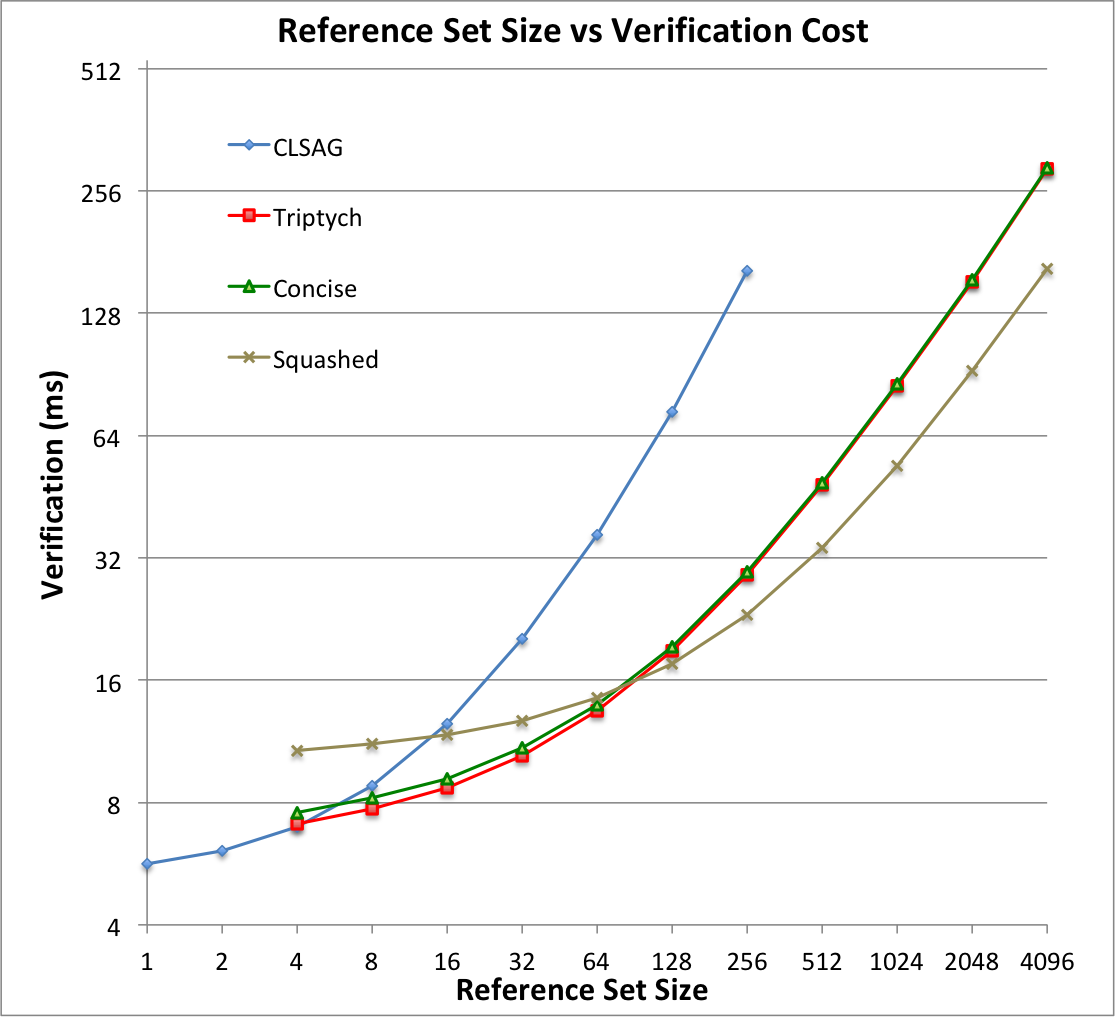
\includegraphics[width=8cm]{figures/refset_1batch_ver.png}
    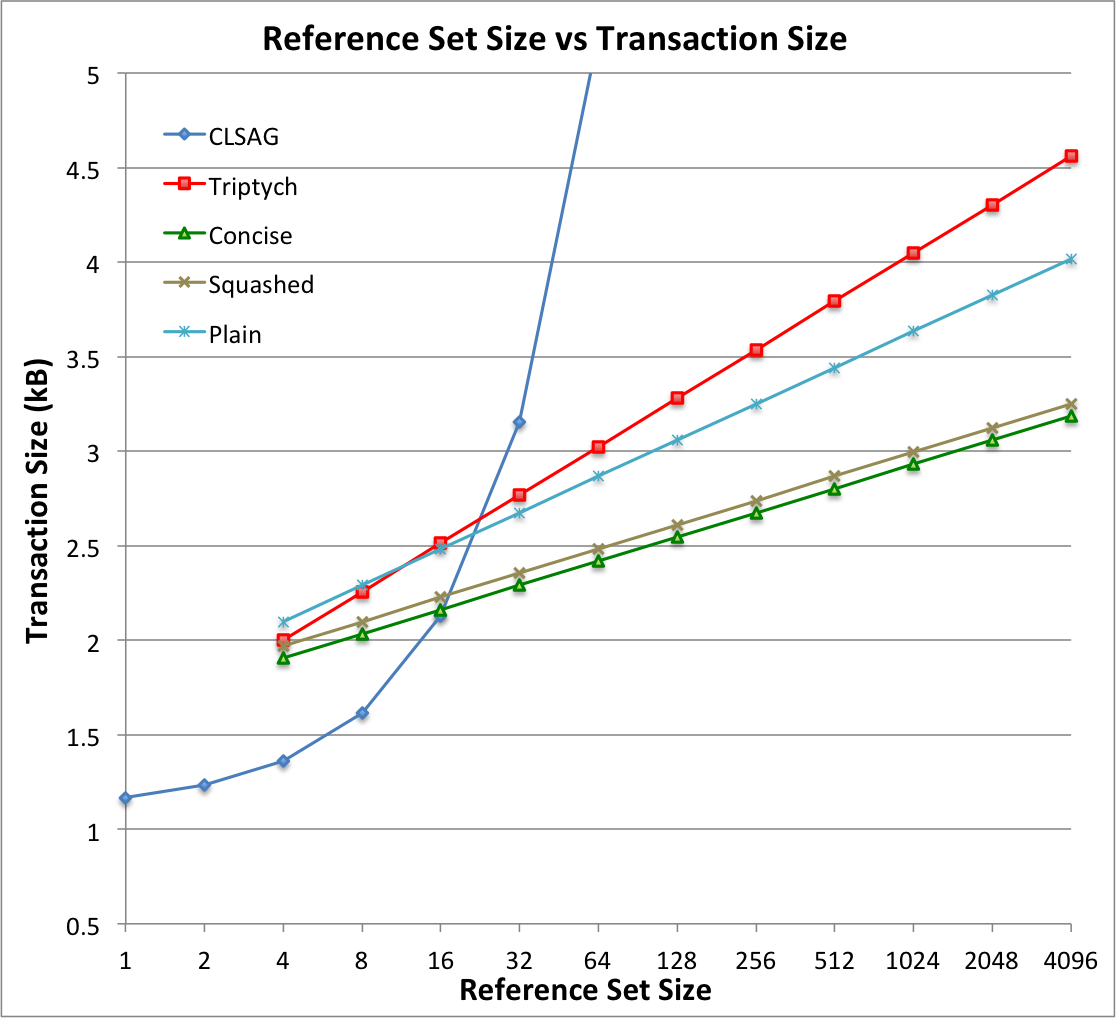
\includegraphics[width=8cm]{figures/refset_1batch_size.png}
    \captionof{figure}{[Left] Membership proof reference set size vs verification cost for 2-input/2-output transactions and no batch-verification. Note that both axes are logarithmic.}
    \label{figure:efficiency-refsetsize-ver}
    \captionof{figure}{[Right] Membership proof reference set size vs verification size for 2-input/2-output transactions and no batch-verification.}
    \label{figure:efficiency-refsetsize-size}
\end{center}

In Figure \ref{figure:efficiency-refsetsize-ver} we see that Seraphis-Concise and Triptych have practically identical verification costs. This is because the modifications to Triptych to get Concise-Grootle proofs have minimal effect on verification costs when reference sizes are reasonably large, and because Seraphis composition proofs have negligible verification cost compared to Concise-Grootle proofs.

Seraphis-Plain is only marginally faster than Seraphis-Concise (less than 10\%), because the verification optimizations that can be used by Seraphis-Plain are relatively inefficient.\footnote{For those readers familiar with Lelantus-Spark's Grootle proofs, we used 2-byte weights to aggregate keys during verification.}

We also see that above reference set size 4, CLSAG performs significantly worse than Seraphis-Concise and Triptych. The performance costs of CLSAG for `large' reference set sizes (above around 5-15) is the driving motivator behind research into protocols like Triptych and Seraphis.

It would seem that Seraphis-Squashed is unfavorable below a reference set size of 128, but Figures \ref{figure:efficiency-refsetsize-ver-25batch} and \ref{figure:efficiency-16inout-ver} will expose the advantages of that protocol variant.

Figure \ref{figure:efficiency-refsetsize-size} further reinforces the costliness of CLSAG, and reveals that Seraphis transaction sizes scale better than Triptych with reference set sizes, which is thanks to the relative simplicity of Concise-Grootle proofs. Here we also see that the marginal performance gains of Seraphis-Plain compared to Seraphis-Concise come at a significant transaction size cost.

\begin{center}
    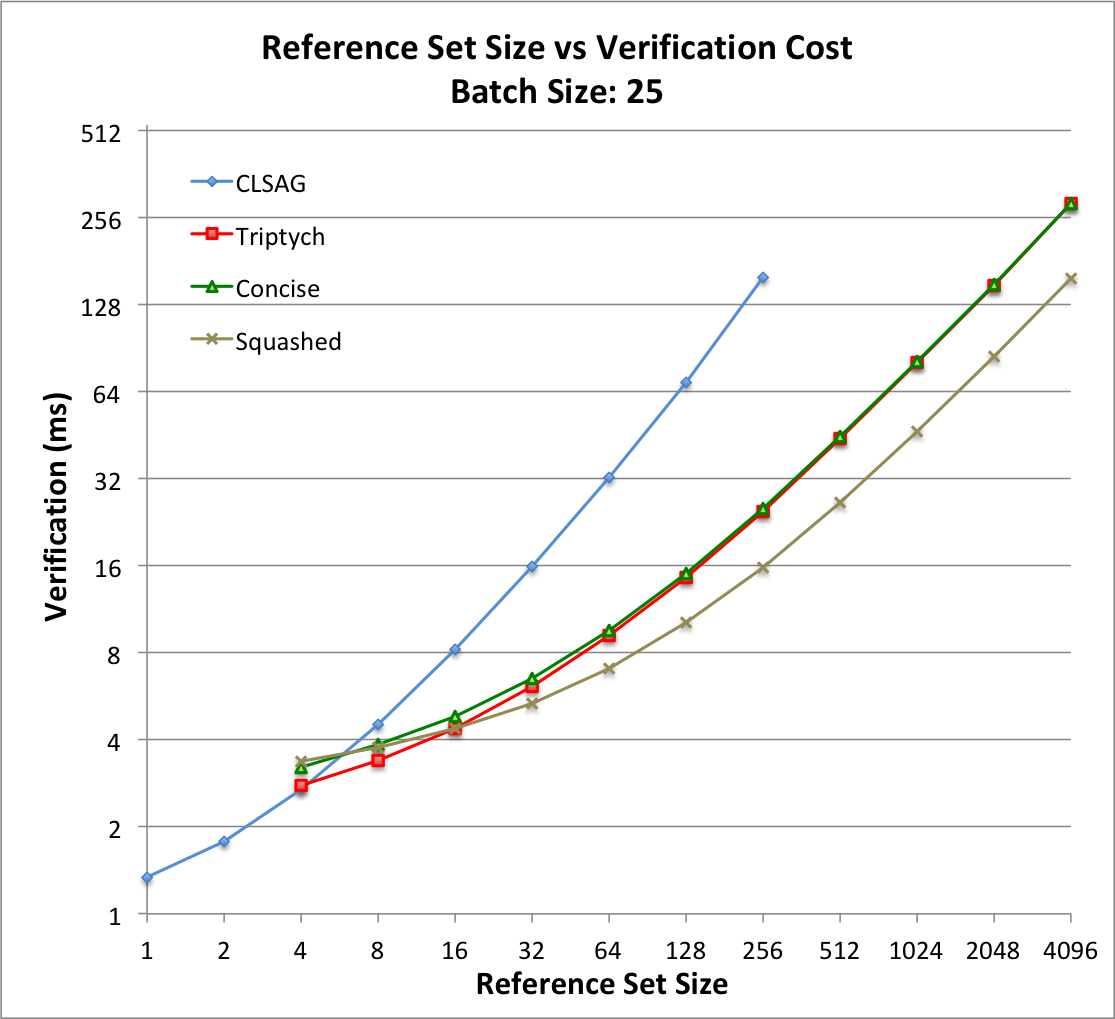
\includegraphics[width=8cm]{figures/refset_25batch_ver.png}
    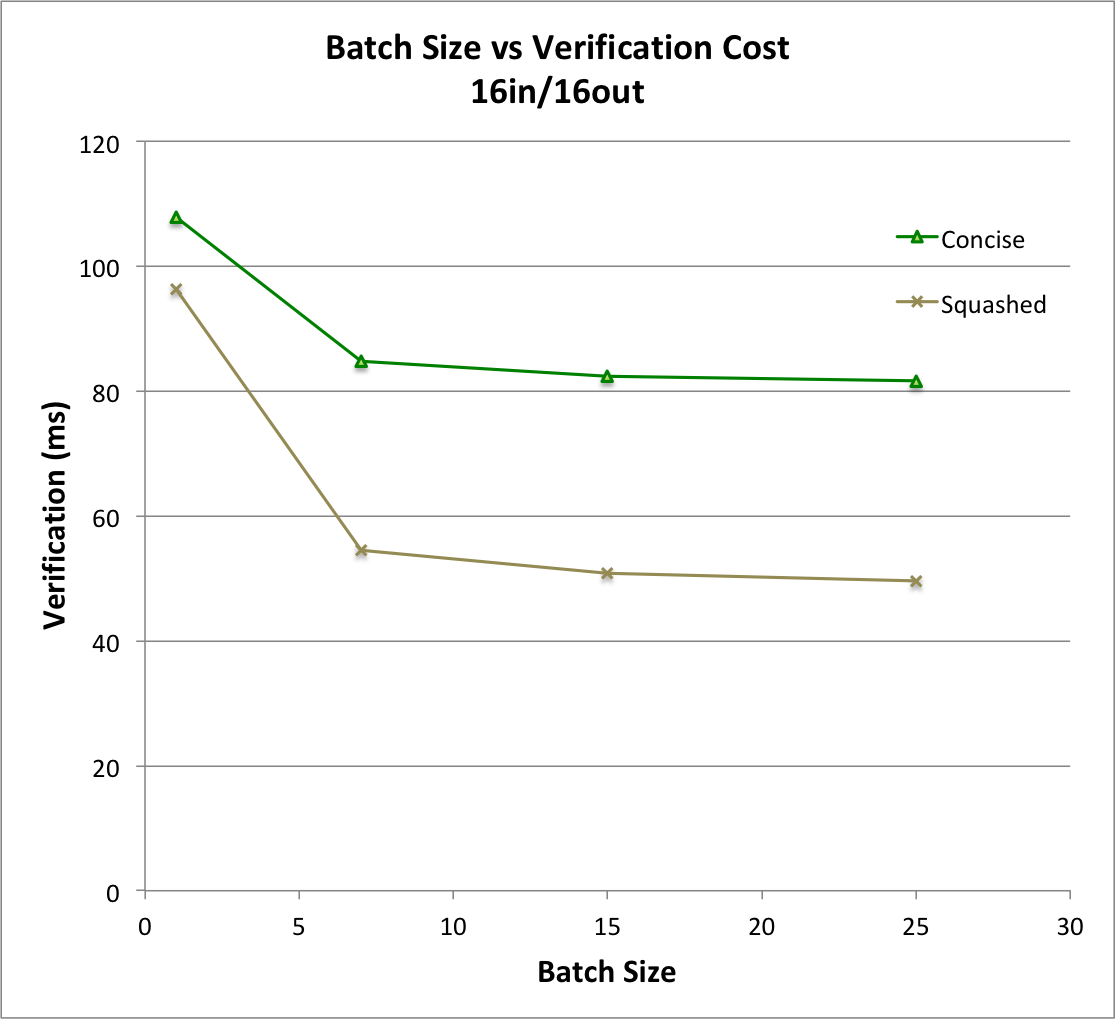
\includegraphics[width=8cm]{figures/16inout_ver.png}
    \captionof{figure}{[Left] Membership proof reference set size vs per-transaction verification cost for 2-input/2-output transactions verified in batches of 25. Note that both axes are logarithmic.}
    \label{figure:efficiency-refsetsize-ver-25batch}
    \captionof{figure}{[Right] Batch size vs per-transaction verification cost for 16-input/16-output transactions with 128-member reference sets.}
    \label{figure:efficiency-16inout-ver}
\end{center}

Figures \ref{figure:efficiency-refsetsize-ver-25batch} and \ref{figure:efficiency-16inout-ver} show what happens when transactions are verified in batches. Multiple Grootle proofs can be verified together in batches, and likewise the aggregated Bulletproofs+ range proofs in a transaction can be batch-verified with range proofs from other equivalent transactions.

Notably, Seraphis-Squashed's performance relative to the other protocols improves greatly when batching is done. This is because Seraphis-Squashed trades simpler membership proofs for range proofs on input image masked amount commitments, and because Bulletproofs+ proofs benefit more from batching than Grootle proofs.\footnote{Grootle proof and Bulletproofs+ proof verification use so-called `multiexponentiation'. It turns out the multiexponentiation operations of those proofs can be combined into one operation, which is a slight optimization (on the order of 1-10\% for unbatched verification).}

\begin{center}
    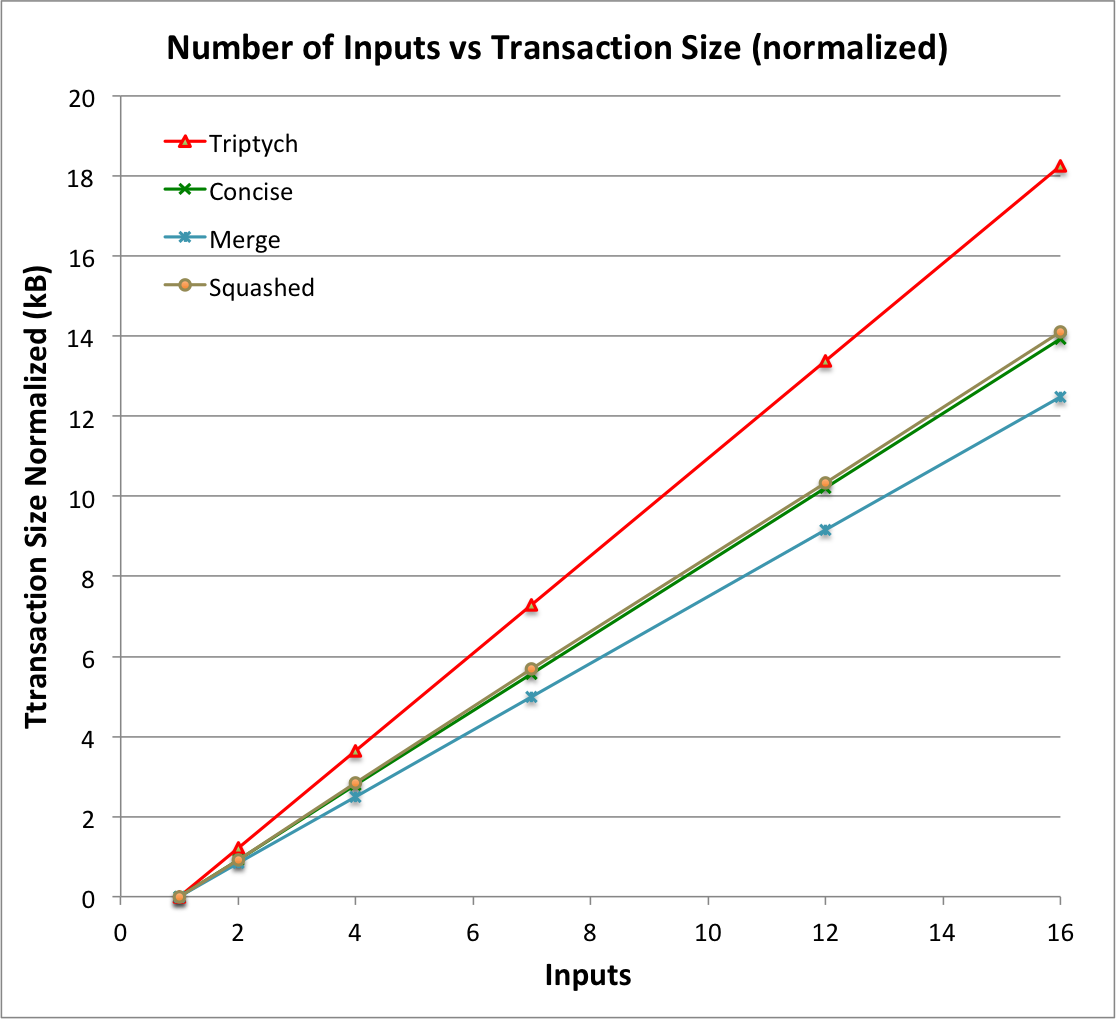
\includegraphics[width=8cm]{figures/inputs_size.png}
    \captionof{figure}{Input count vs transaction size (normalized to the 1-input case) for 2-output transactions with 128-member reference sets and no batch-verification.}
    \label{figure:efficiency-inputs-size}
\end{center}

Finally, in Figure \ref{figure:efficiency-inputs-size} we see how Seraphis-Merge differs from the other variants. In explicit terms, Seraphis-Merge is $32*(1 + 3*(\textrm{num\_inputs} - 1))$ bytes smaller than Seraphis-Concise. Also note that Triptych transaction sizes scale worse with input counts than the Seraphis variants. Even Seraphis-Plain scales better than Triptych with increasing input counts.
